\label{sec:cnn-image}
\subsection{Image Constituents}
For this study, jets clustered the anti-$k_t$ jet algorithm~\cite{Cacciari:2008gp}
are used and are required to have $|\eta|<2.1$ such that they remain fully within the
tracker coverage.
For reconstruction study, three types of constituents for jet image formations
are considered: tracks, calorimeter clusters and calorimeter towers. The truth level images
based on truth particles are also considered as performance benchmark as they have
higher qualities than images based on reconstructed quatities which are degraded by
finite detector resolution and noise. 

\subsubsection{tracks}
Track reconstructions follow the same procedure as described in Chapter\ref{chap:reconstruction}. Tight quality
criteria~\cite{ATL-PHYS-PUB-2015-051} on the track properties are used to mitigate the impact of pile-up as well as
to reject spurious (fake) tracks that result from multiple charged particles or noise.
Tracks used for this study are required to have $p_\text{T} > 0.5~\GeV$ and to originate from the hard-scatter primary vertex. 
Tracks are assigned to primary vertices based on the track-to-vertex matching resulting from the vertex reconstruction.
Tracks not included in vertex reconstruction are assigned to the nearest vertex based on the
distance $|\Delta z \times \sin\theta|$, up to a maximum distance of 3 mm.
The track to jet association scheme is ghost-association same as documented in Sec.\ref{sec:vbf-objsel}.


\subsubsection{calorimeter clusters}
The first type of energy information considered is topological calorimeter-cell 
clusters (topo-clusters)~\cite{Aad:2016upy}.
The algorithm uses as seeds calorimeter cells
with energy significance $|E_\text{cell}|/\sigma_\text{noise}>4$,
iteratively combines all neighbouring cells with
$|E_\text{cell}|/\sigma_\text{noise}>2$ and finally adds neighbouring cells
without any significance requirement.
%Topo-clusters at the EM scale are used as input for jet reconstruction with 
%with distance parameter $R=0.4$, as provided by FastJet~\cite{Cacciari:2011ma}.  

\subsubsection{calorimeter towers}
An alternative energy organization scheme, calorimeter towers,
is used to associate calorimeter information with the jets
reconstructed from topo-clusters.
Calorimeter towers are fixed-size objects ($\Delta\eta\times\Delta\phi=0.1\times0.1$)~\cite{cscbook}
that ensure a uniform segmentation of the calorimeter information.
Instead of building clusters, the cells are projected onto a fixed grid in $\eta$ and $\phi$ corresponding to 6400 towers
for the full calorimeter coverage $|\eta|<5$.
Calorimeter cells which completely fit within a tower contribute their total energy
to the single tower.
Cells which extend beyond the tower boundary contribute to multiple
towers, depending on the overlap fraction of the cell area with the towers.
In the following, towers are matched geometrically to jets built from topo-clusters, by considering all the towers within
the jet radius $R=0.4$.

%An overall jet calibration corrects the detector-level jet $p_\text{T}$ to the particle-level jet $p_\text{T}$ on average~\cite{Aad:2014bia}.   
\subsubsection{truth particles}
Truth-particle jets in Monte Carlo (MC) simulation are built from generated stable particles with a mean lifetime $\tau>30$~ps, 
excluding muons and neutrinos.
As with the detector-level jets, truth-particle jets are clustered with the anti-$k_t$ $R=0.4$ algorithm.
The $p_\text{T}$ of the truth-particle jet is used to select the jets.
Two $p_\text{T}$ ranges are considered for this study: $150~\GeV<p_\text{T}<200~\GeV$ and $400~\GeV<p_\text{T}<500~\GeV$.


\subsection{Image Formation}

There is an extensive literature on formation of jet images images. In line with the work such as~\cite{Cogan:2014oua,Almeida:2015jua}, the first step in constructing a jet image rotates and Lorentz boost all of the constituents inside a jet so that $\phi_\text{jet}=\eta_\text{jet}=0$. Then, the jet is cropped into a grid of size $16\times 16$ in $\eta$ and $\phi$ with pixel sizes $0.05\times 0.05$ and centered.  The intensity of each pixel is the total $p_\text{T}$ within the pixel, using a particular type of constituents (calorimeter-cell clusters, towers, tracks, or truth particles). Each image is then normalized so that $\sum_i I_i=1$, where $I_i$ is the intensity of the $i^\text{th}$ pixel. Normalization is performed for the tagger to learn only the information orthogonal to the jet transverse momentum.  %Normalization is known to remove useful discrimination information, but studies suggest the impact is small and it is useful for training. For an extensive description of the impact of image preprocessing on the information content of a jet image, see Ref.~\cite{deOliveira:2015xxd}.

One representative set of gluon jet images using different inputs is shown in Figure~\ref{fig:cnn-oneimage} and the average quark and gluon jet images and their differences are shown in Figure~\ref{fig:cnn-avg:truthtrack} and Figure~\ref{fig:cnn-avg:clustertower}. As clearly show, Jet images are extremely sparse. Only when shown in average form would one see a difference between quark and gluon jets in ensemble level. As expected, the radiation pattern around the core is broader for gluon jets relative to quark jets.
The slightly reduced central activity in track images shown in Figure~\ref{fig:cnn-avg:truthtrack} is compatible with the lower track reconstruction efficiency at the core of the jet~\cite{Aaboud:2017all}.
Topo-cluster images are found to be more collimated than tower images (Figure~\ref{fig:cnn-avg:clustertower}) as a result of the built-in noise suppression mechanism that removes some of the soft large-angle radiation.

\begin{figure}[htpb]
\begin{center}
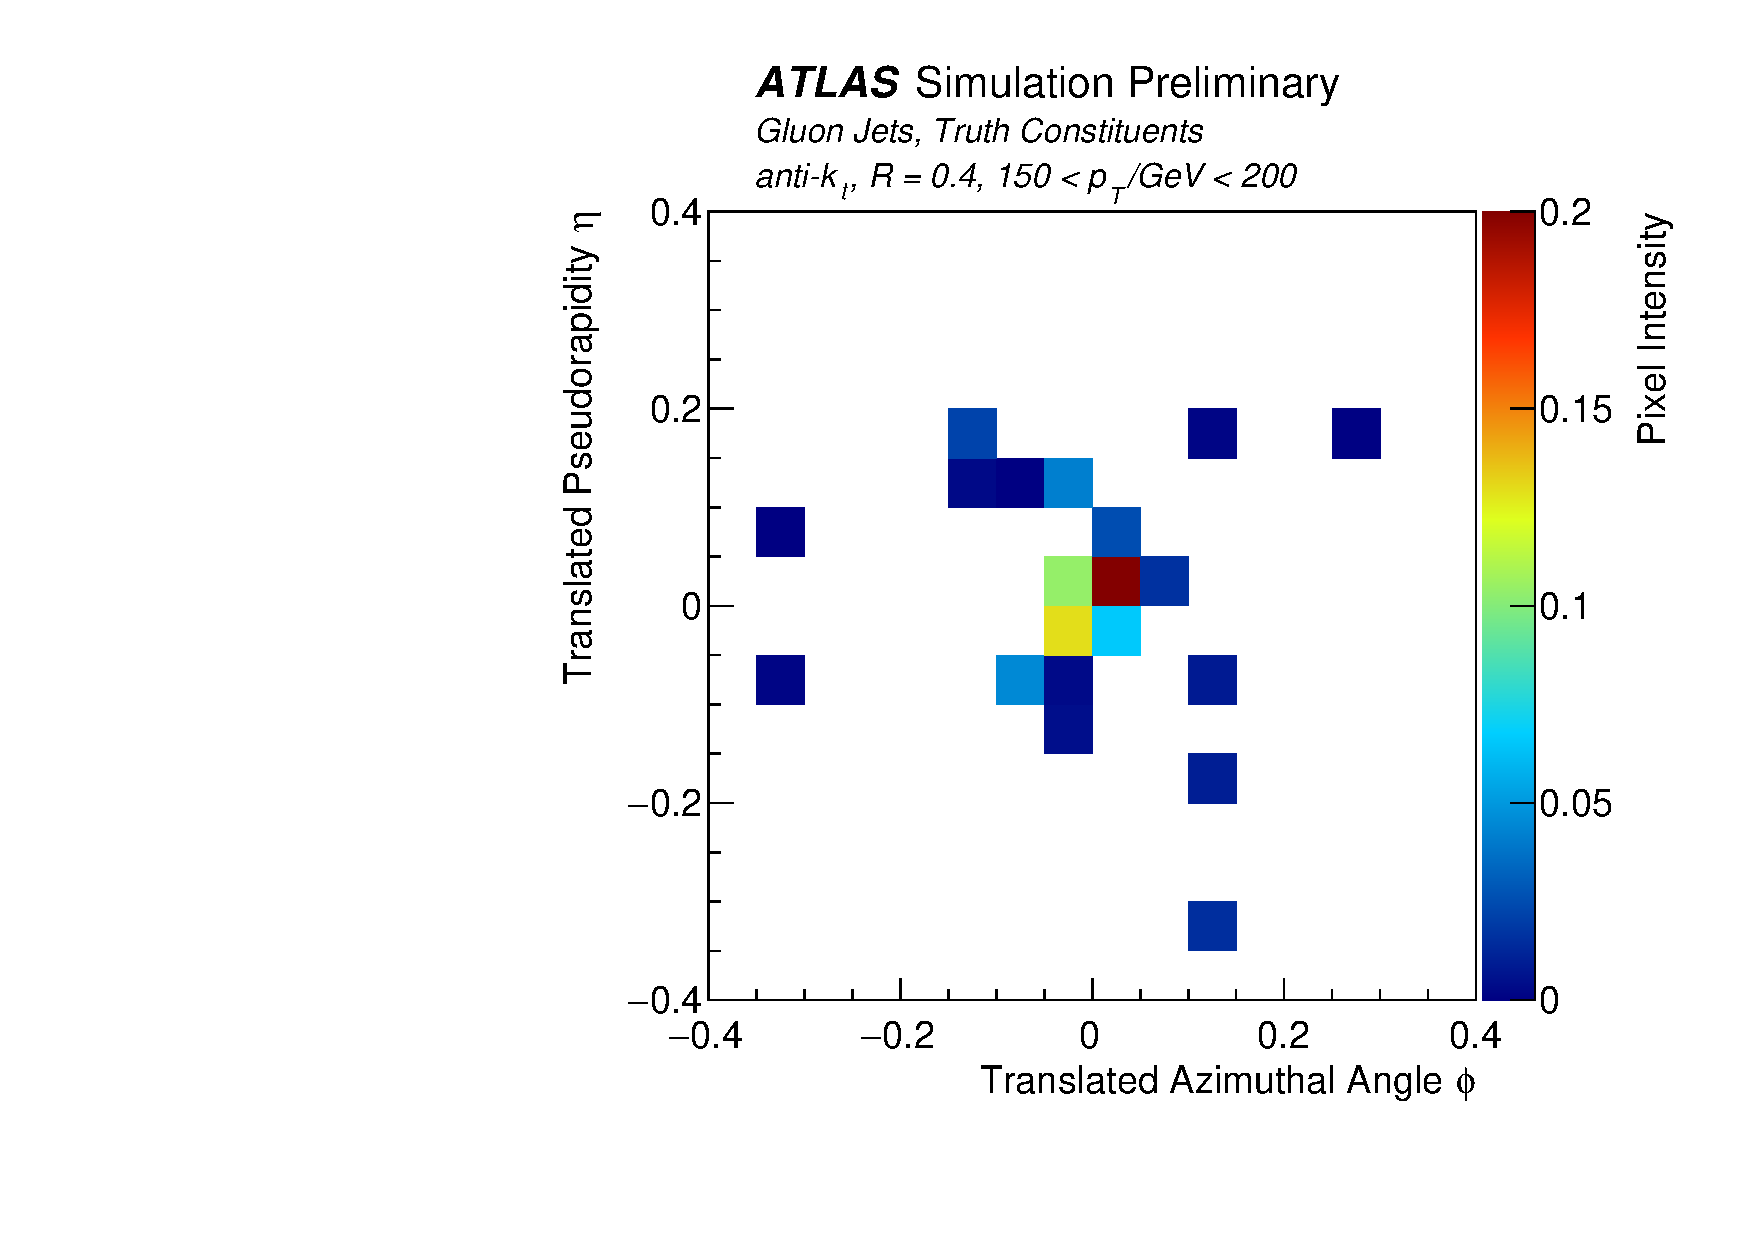
\includegraphics[width=0.45\textwidth]{figures/CNN/gluon_truth_one.pdf}
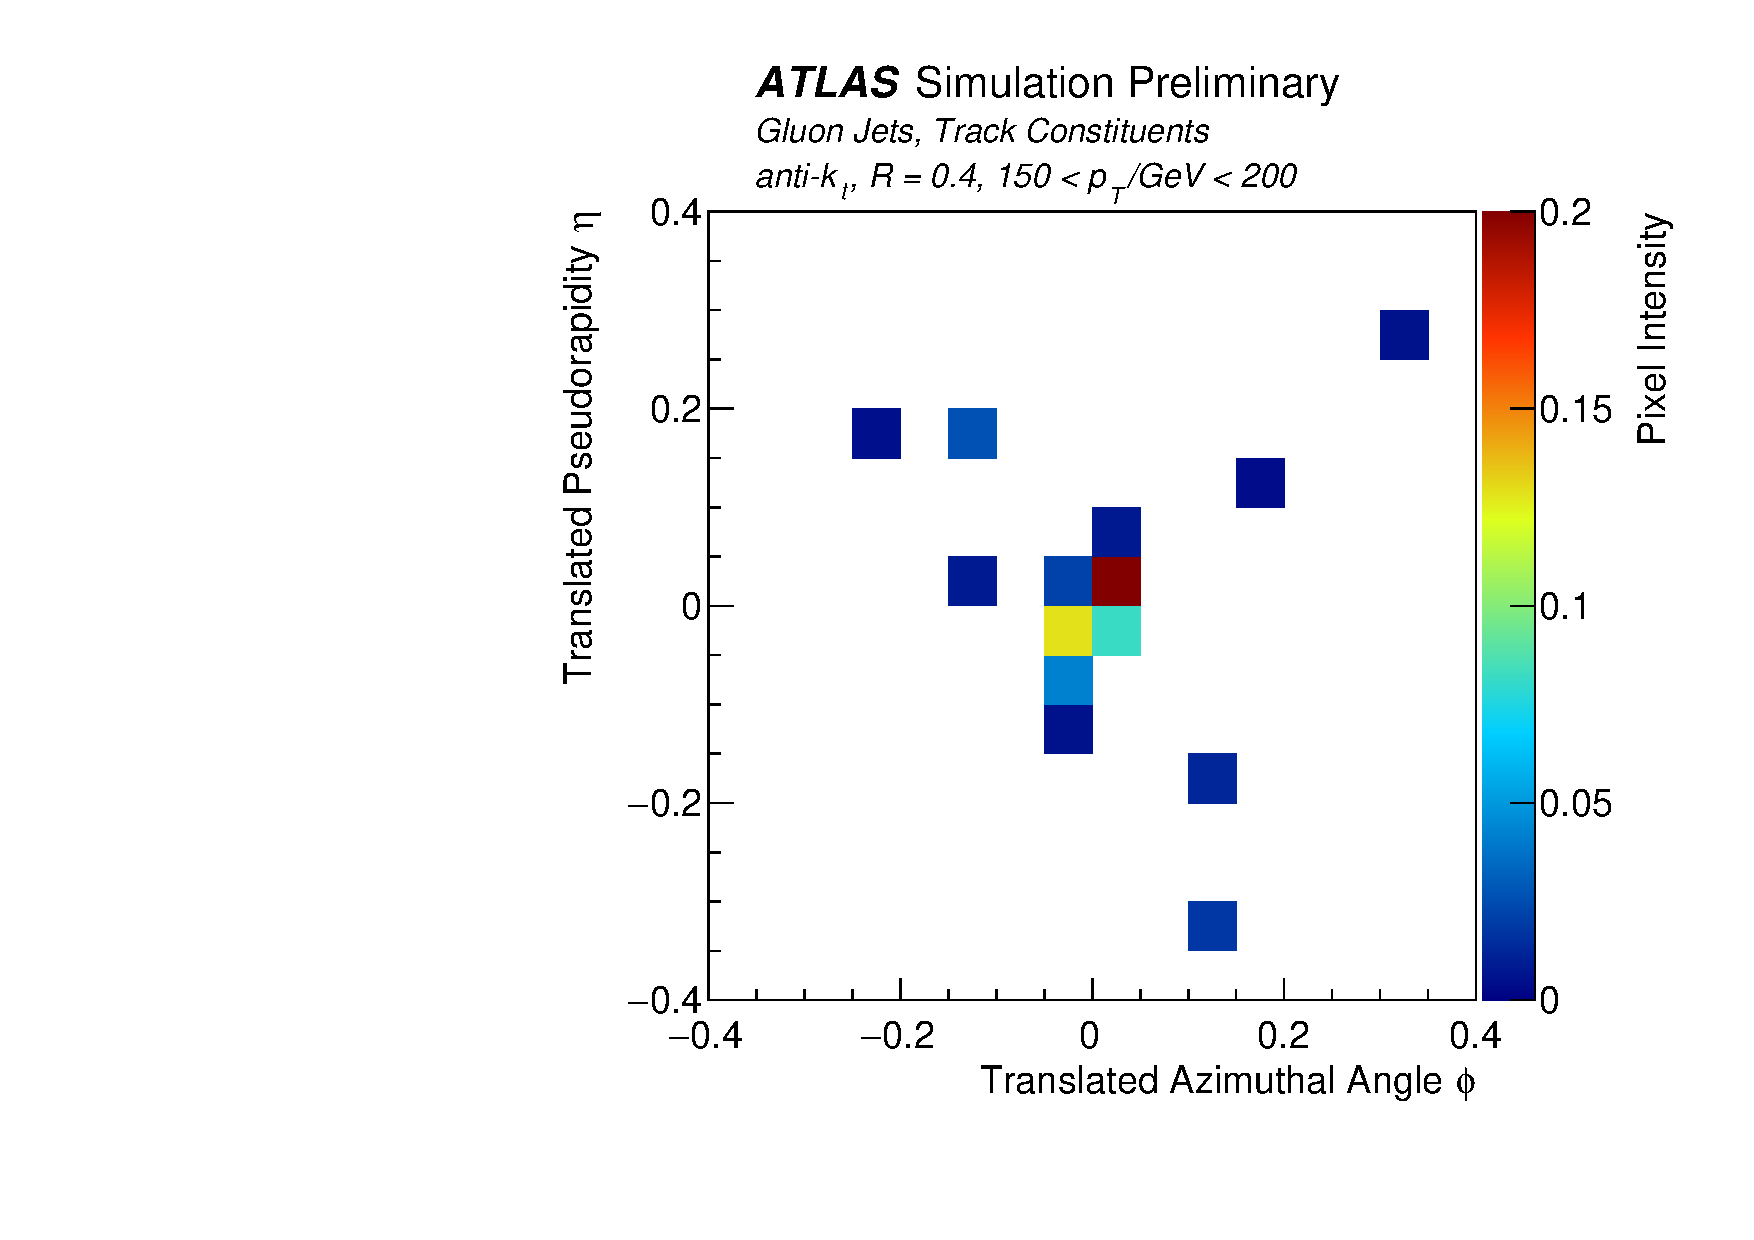
\includegraphics[width=0.45\textwidth]{figures/CNN/gluon_track_one.pdf}\\
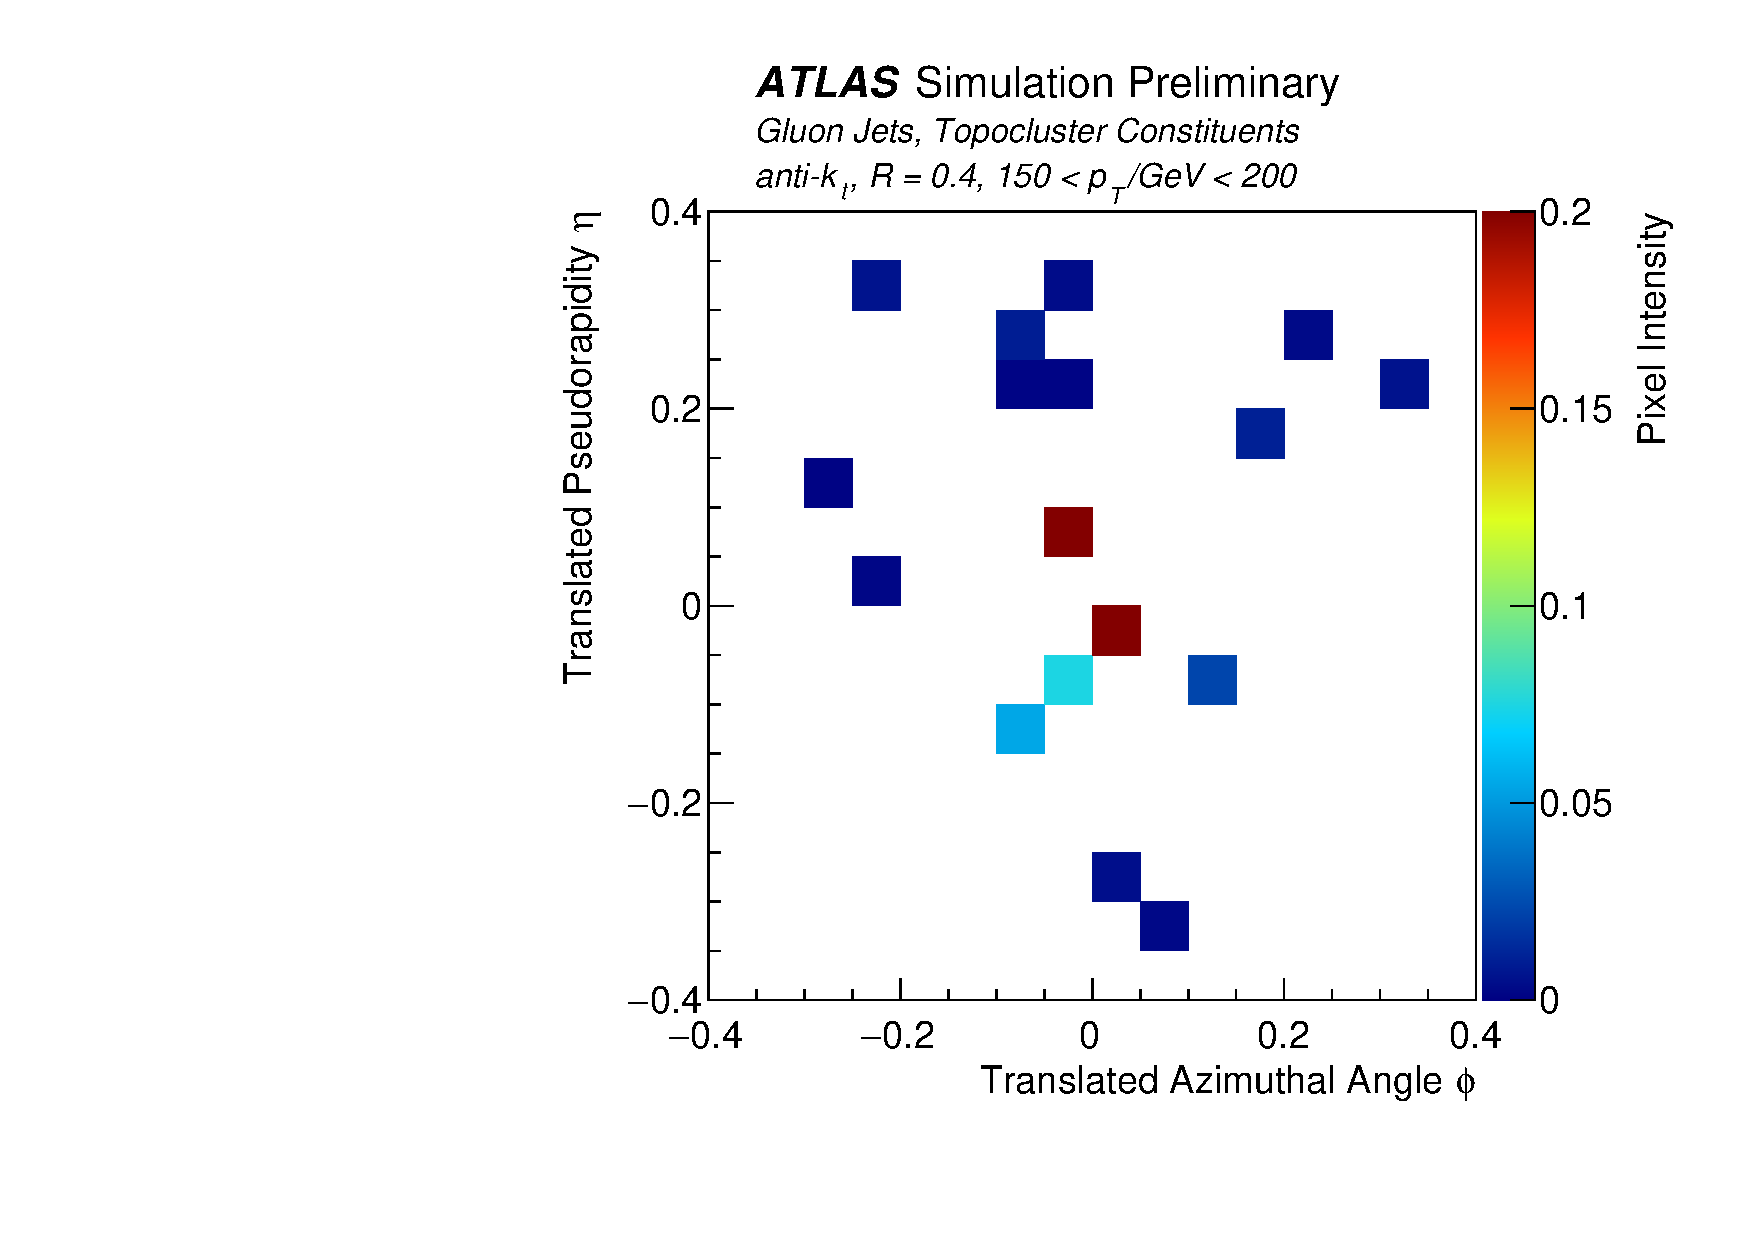
\includegraphics[width=0.45\textwidth]{figures/CNN/gluon_cluster_one.pdf}
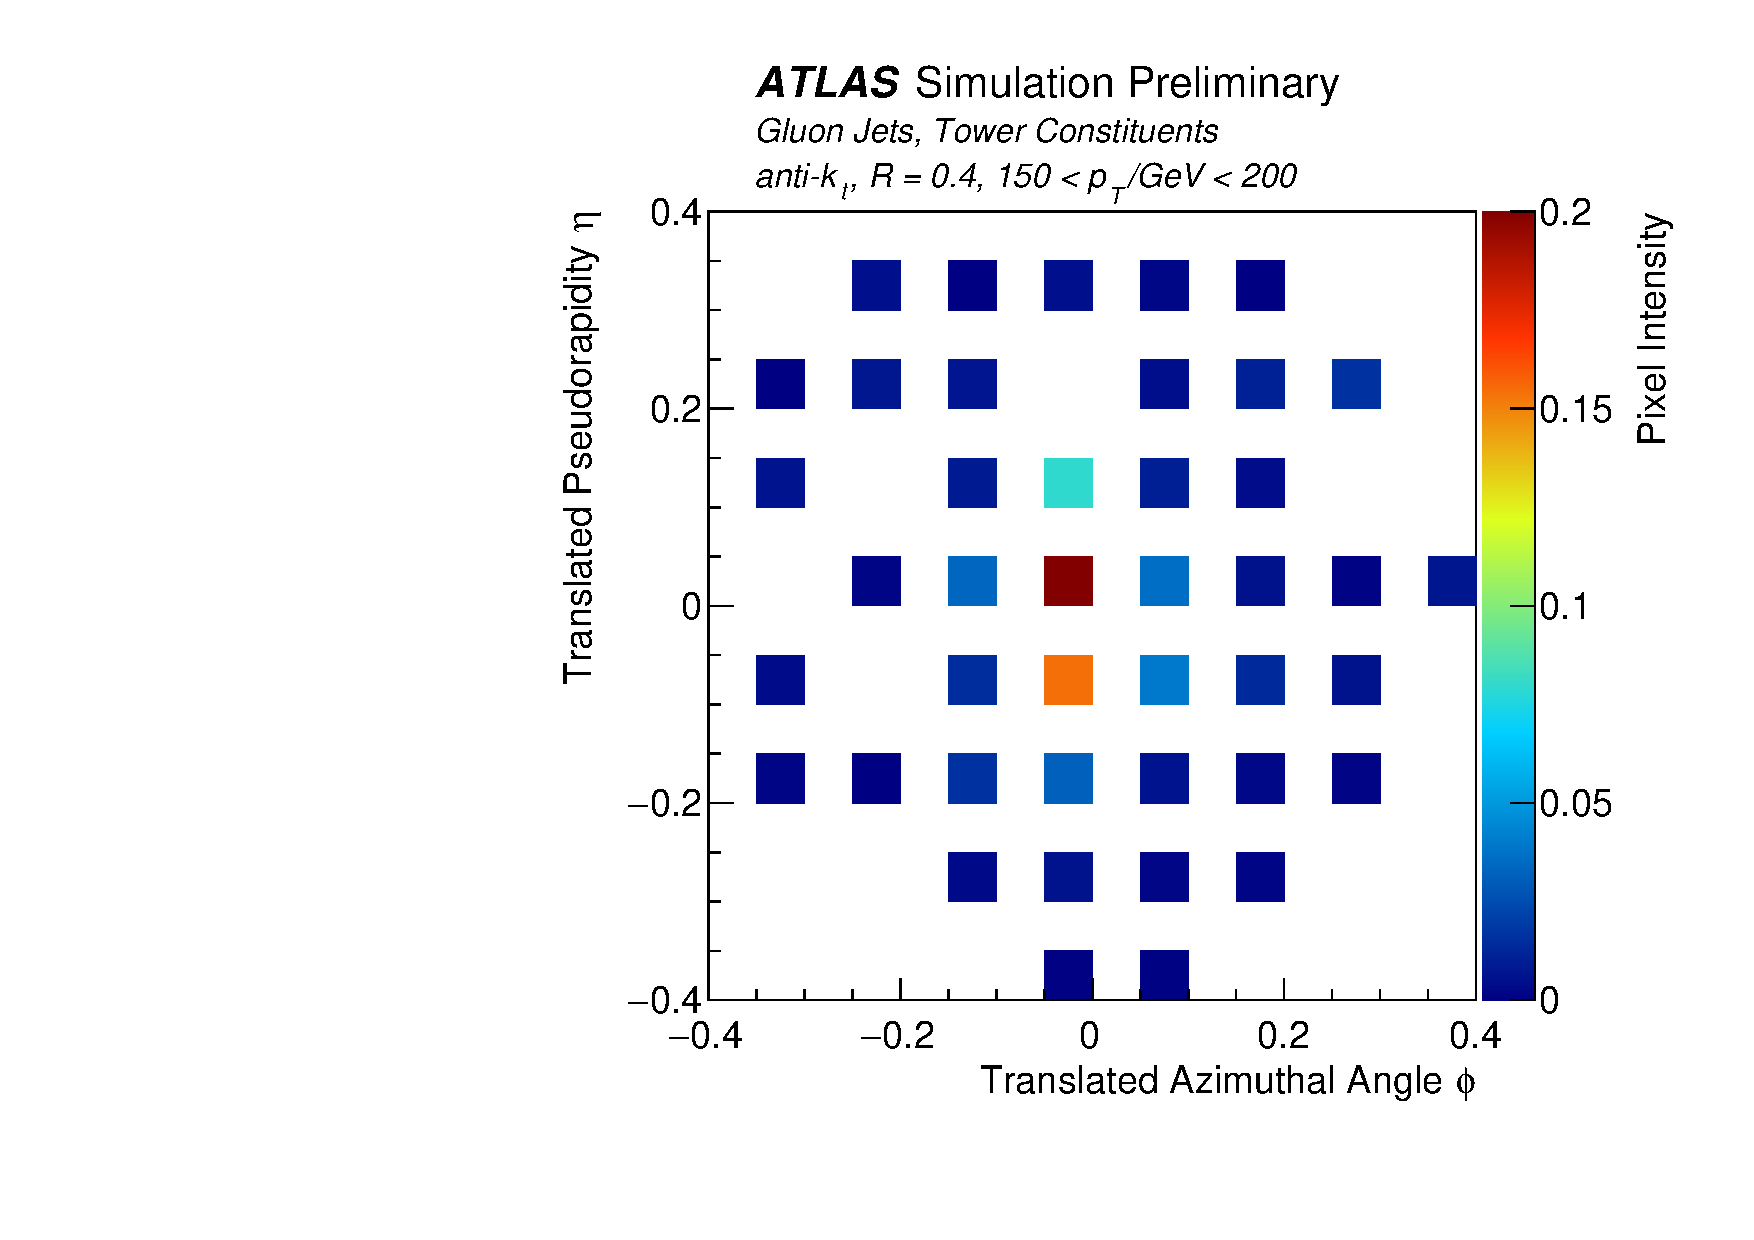
\includegraphics[width=0.45\textwidth]{figures/CNN/gluon_tower_one.pdf}
\caption{The stable particles (top left), track (top right), topocluster (bottom left), and tower (bottom right) images 
for an example gluon jet image.  
The tower image has gaps between hit pixels because the $0.1\times 0.1$ towers are projected onto a $0.05\times 0.05$ jet image.}
\label{fig:cnn-oneimage}
\end{center}
\end{figure}

\begin{figure}[htpb]
\begin{center}
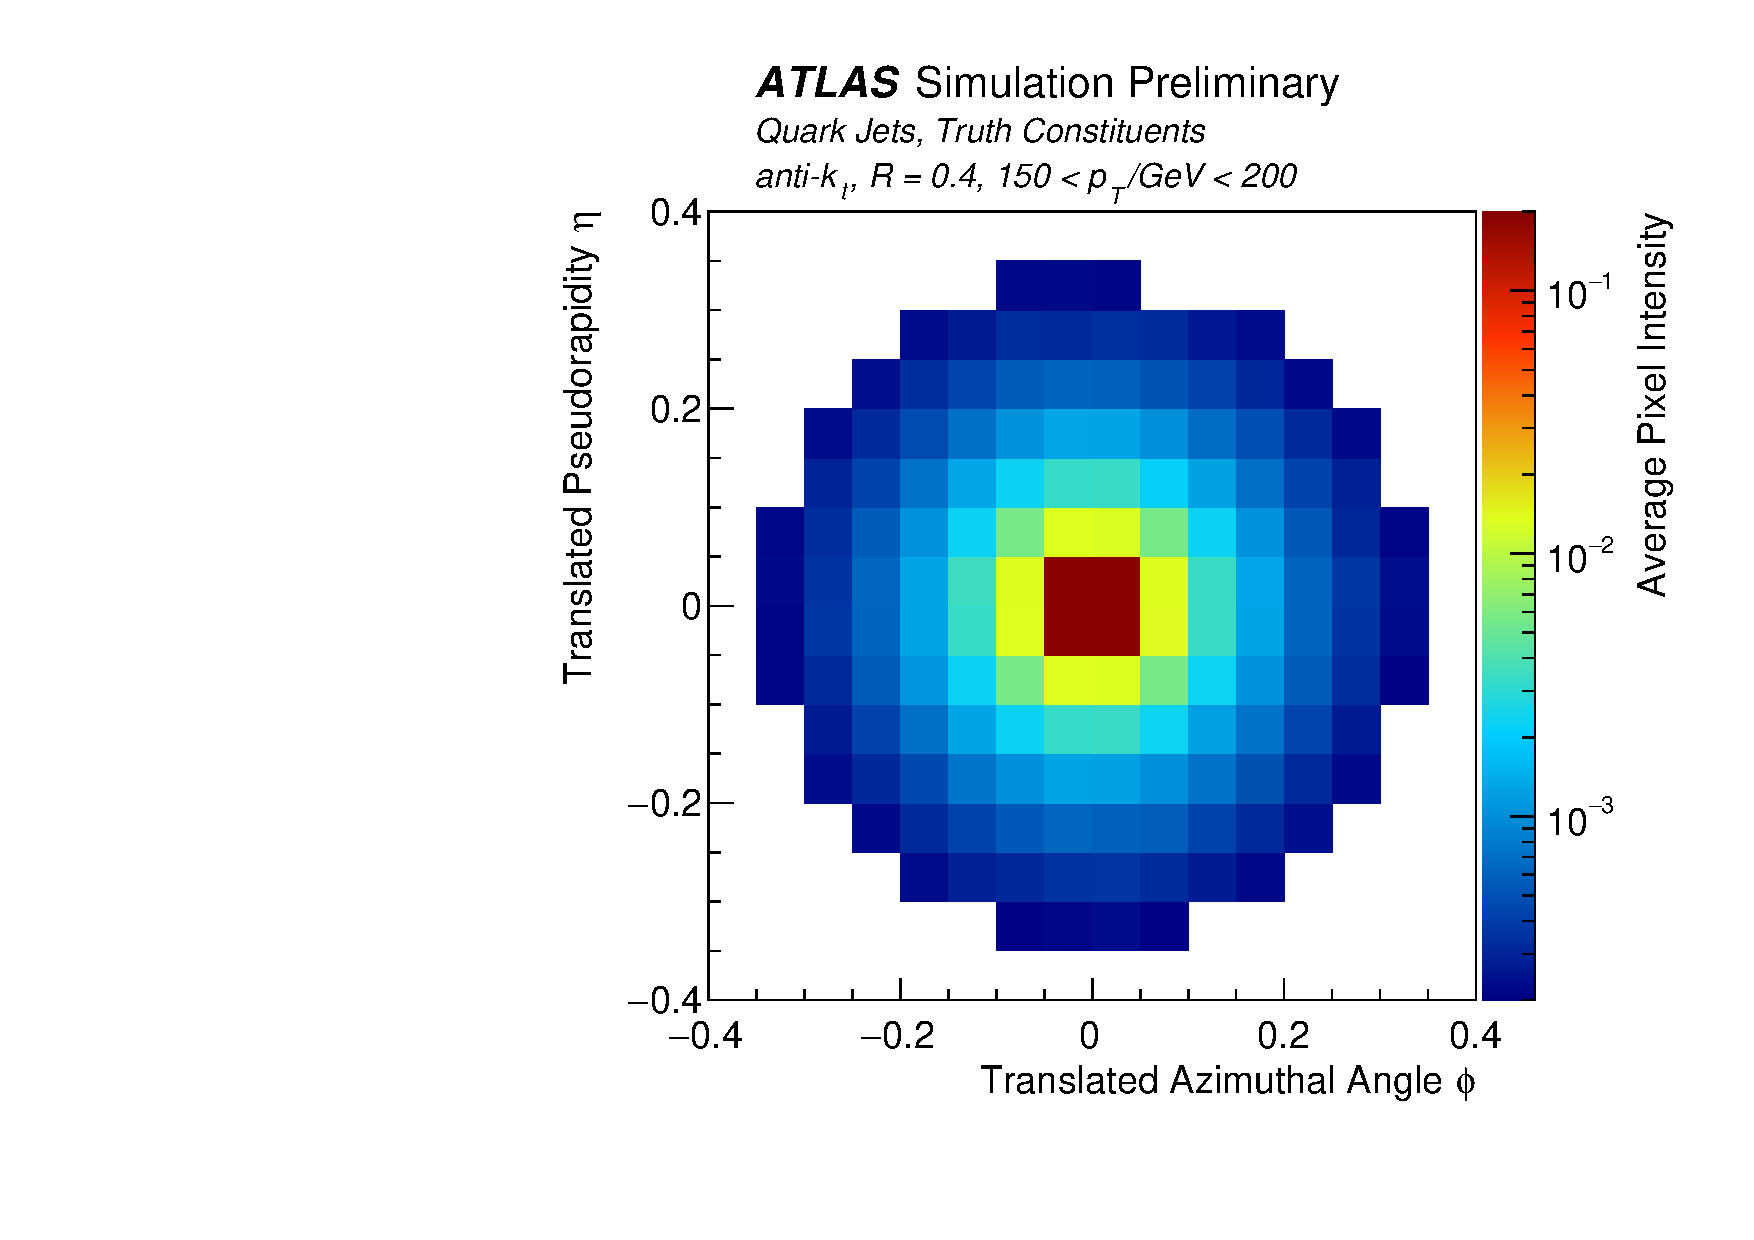
\includegraphics[width=0.31\textwidth]{figures/CNN/quark_truth.pdf}
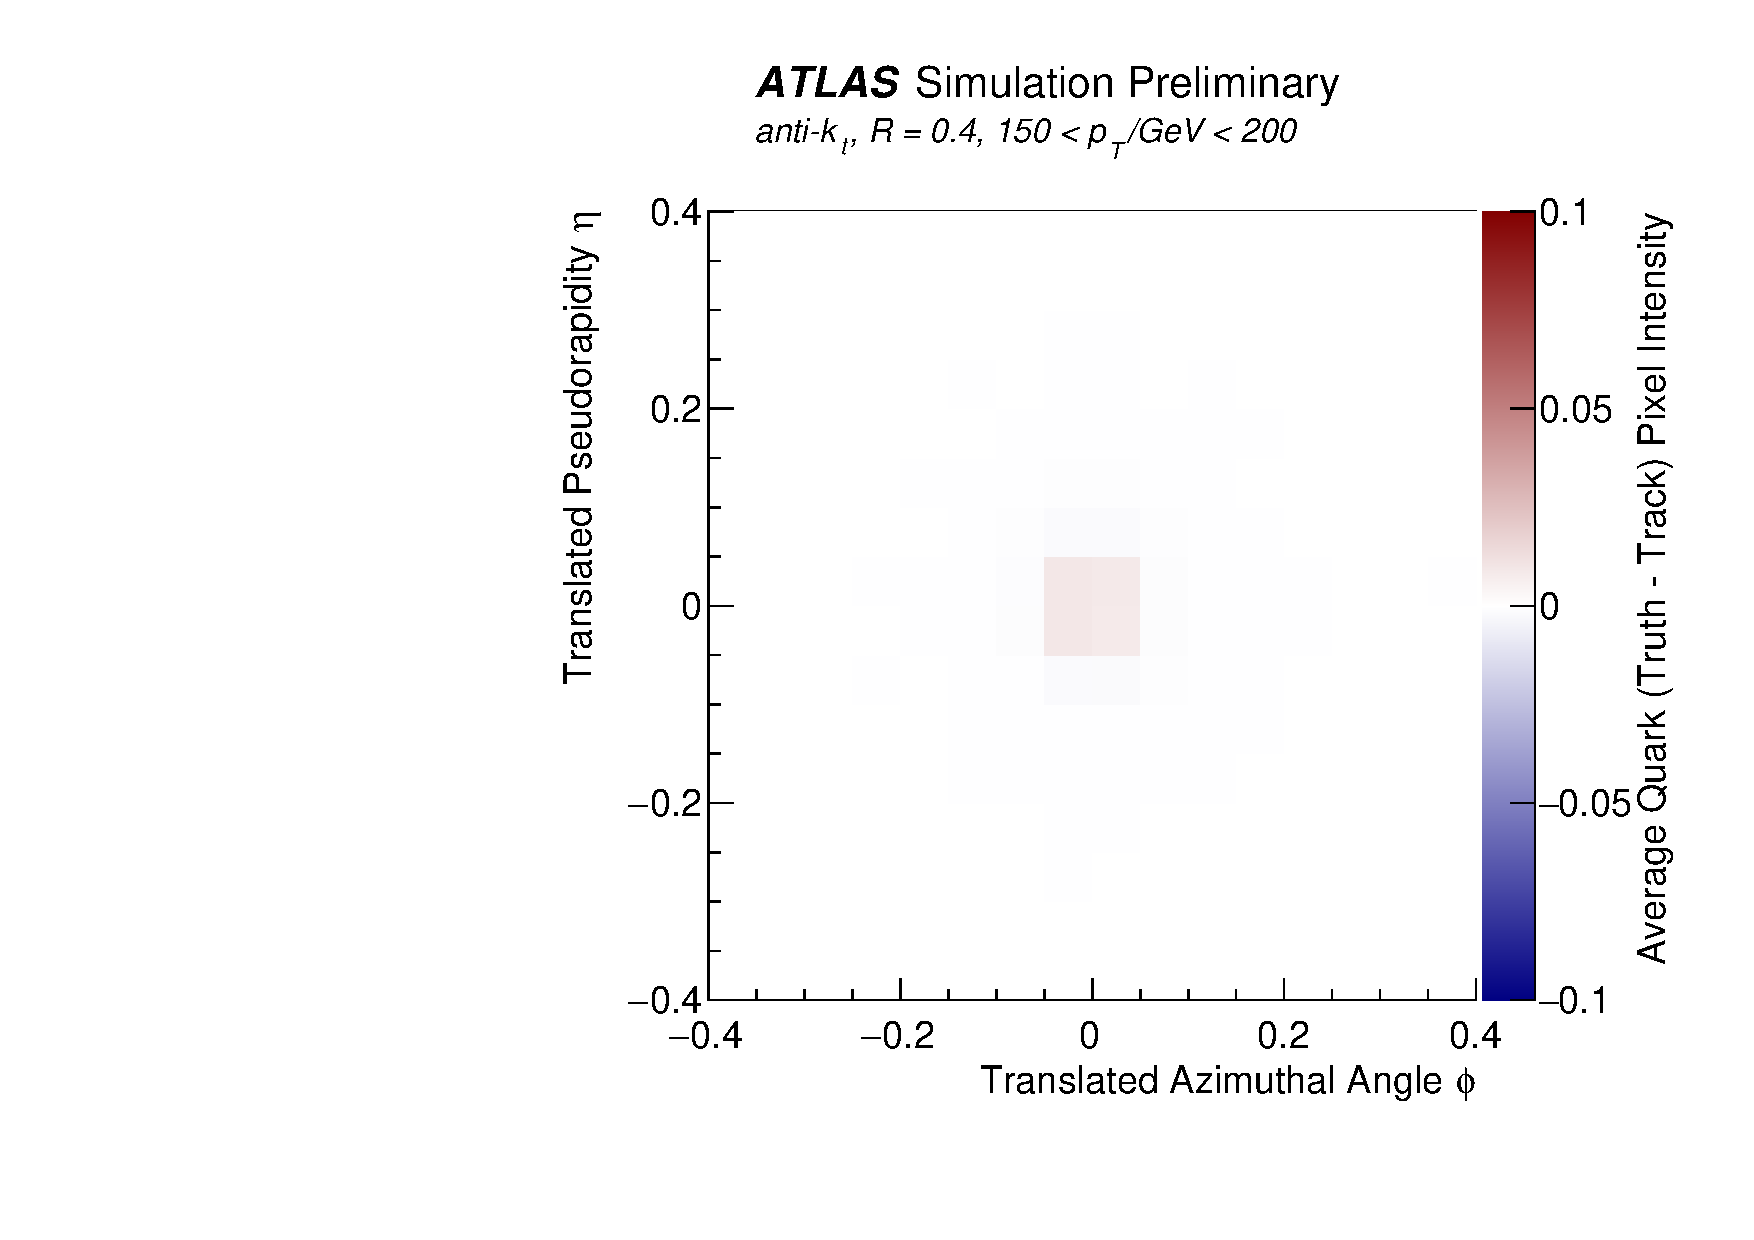
\includegraphics[width=0.31\textwidth]{figures/CNN/diff_quark_truth_track.pdf}
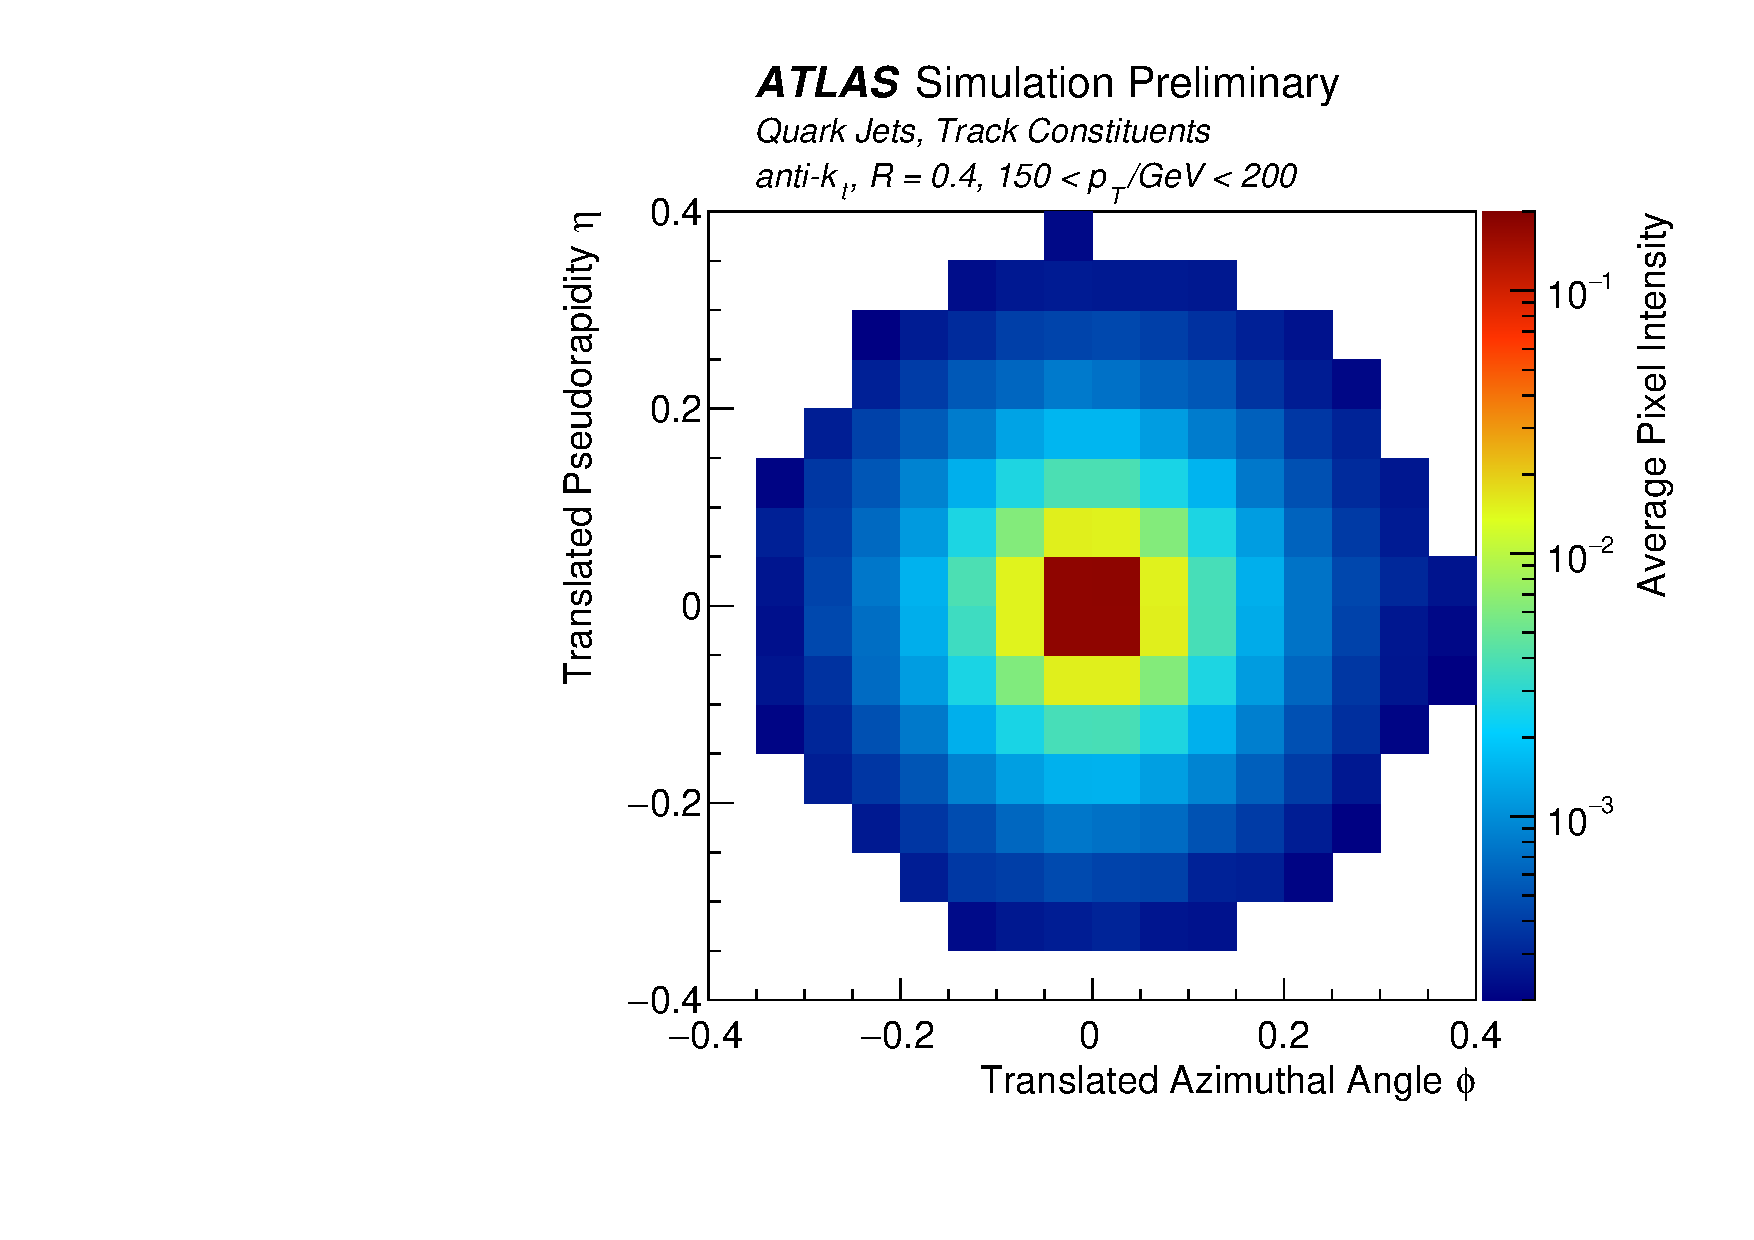
\includegraphics[width=0.31\textwidth]{figures/CNN/quark_track.pdf}\\
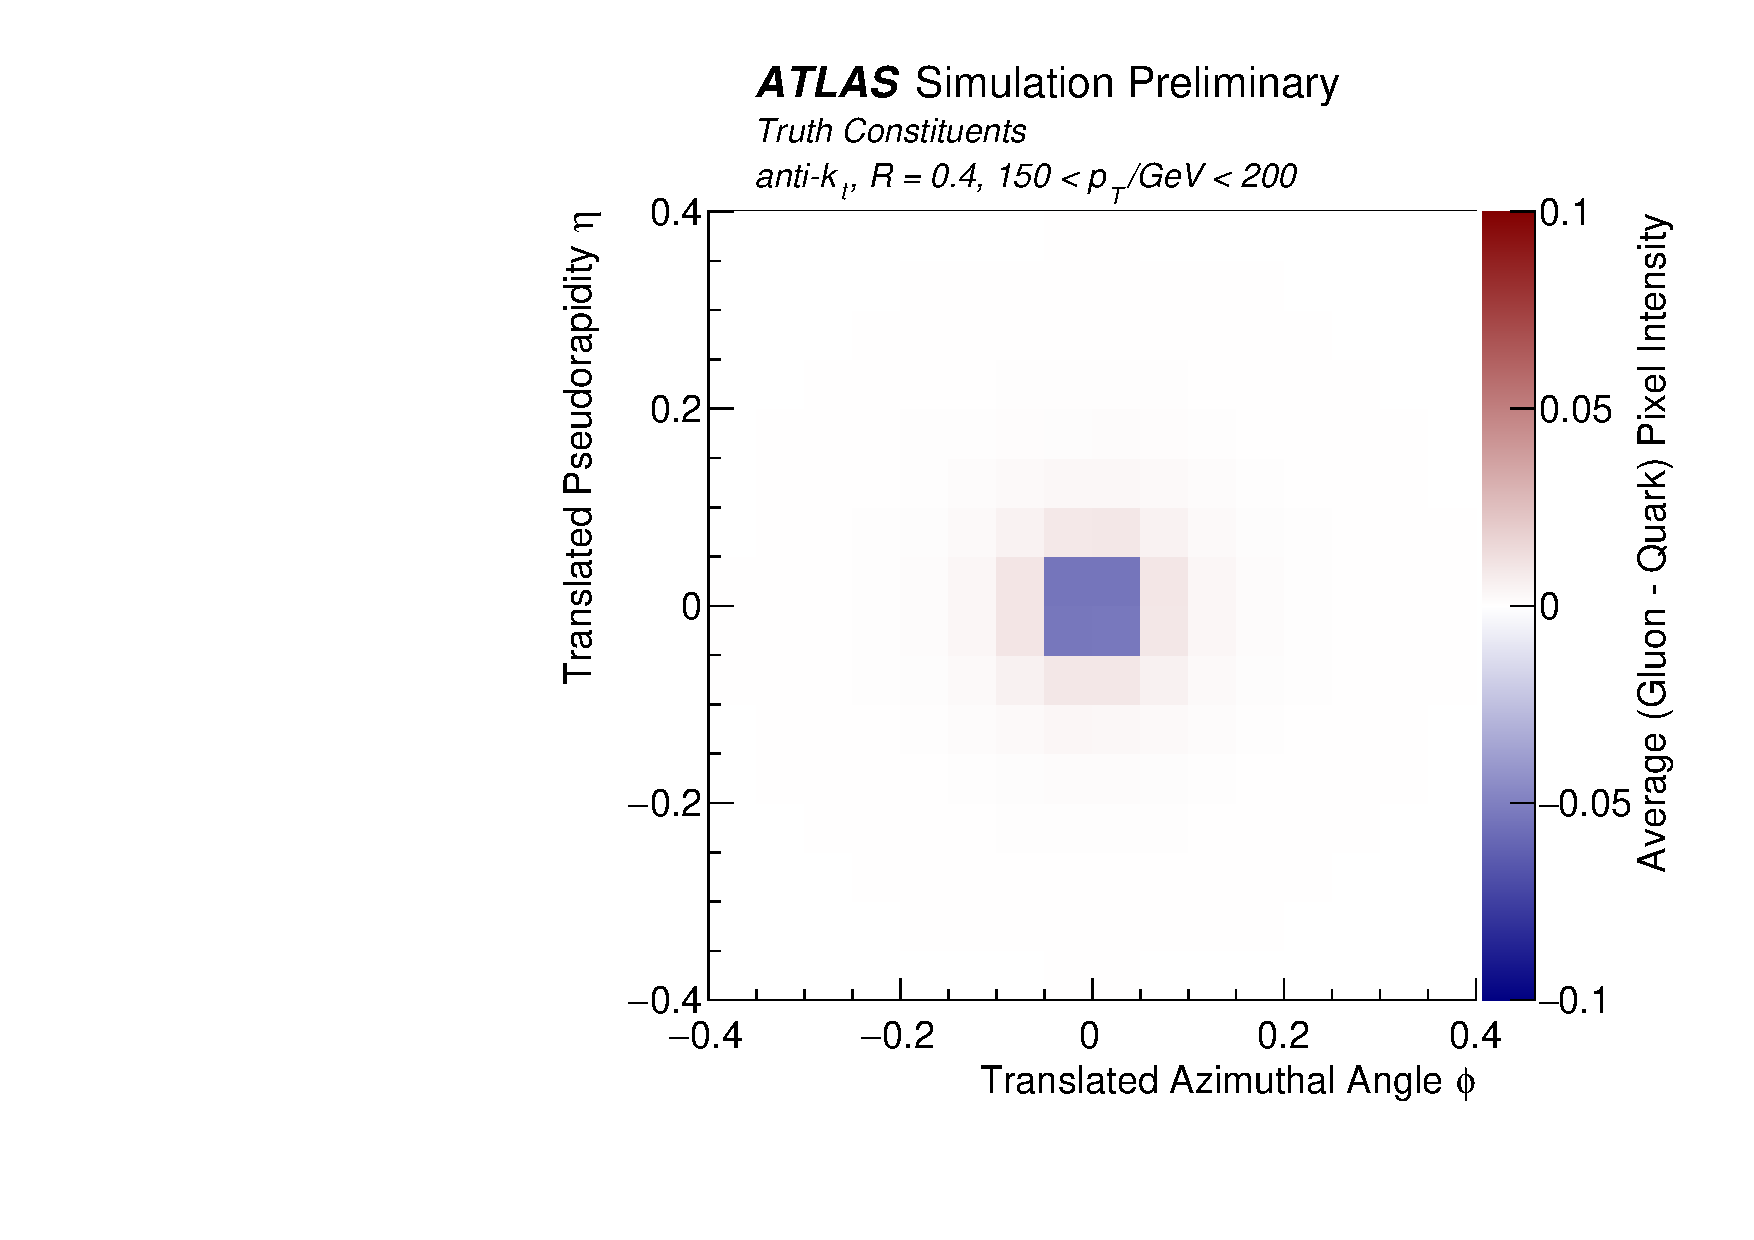
\includegraphics[width=0.31\textwidth]{figures/CNN/diff_truth.pdf}\hspace{54mm}
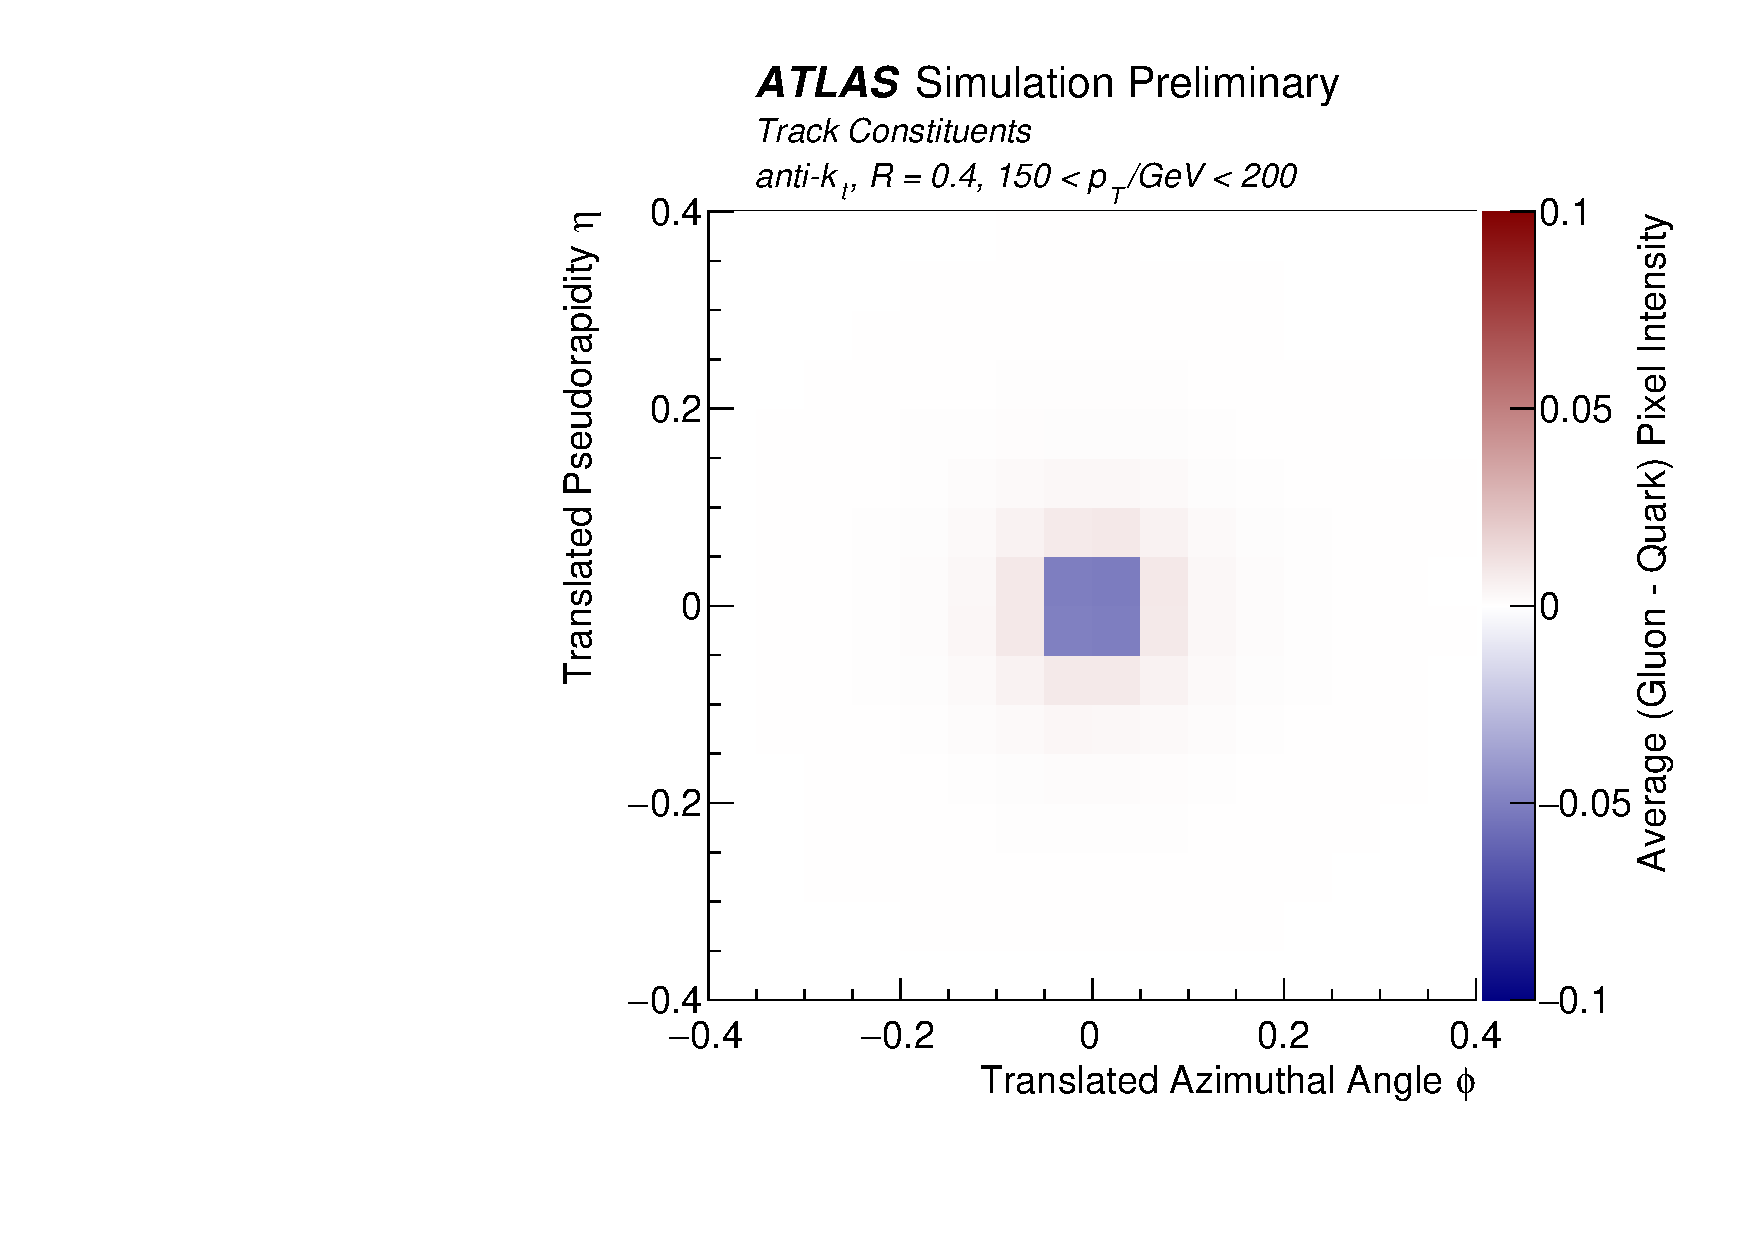
\includegraphics[width=0.31\textwidth]{figures/CNN/diff_track.pdf}\\
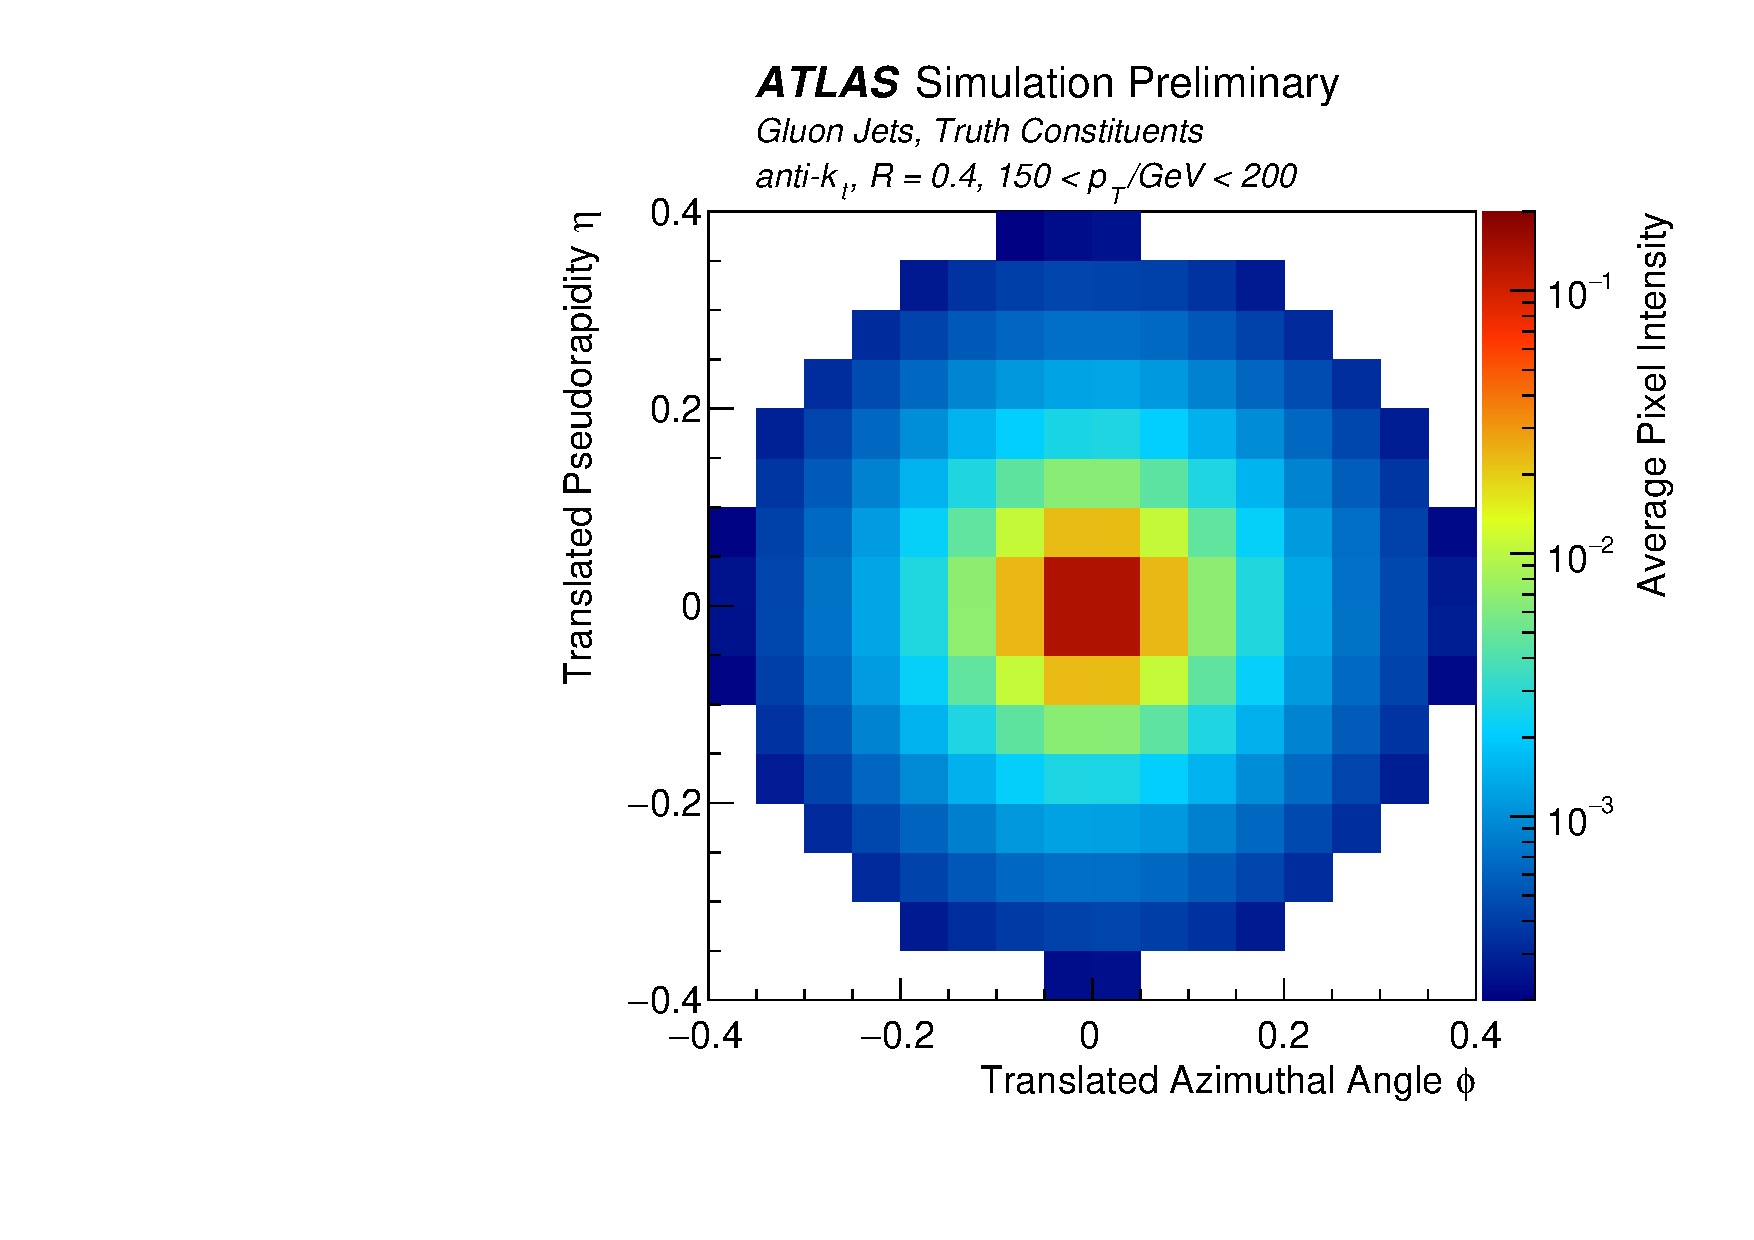
\includegraphics[width=0.31\textwidth]{figures/CNN/gluon_truth.pdf}
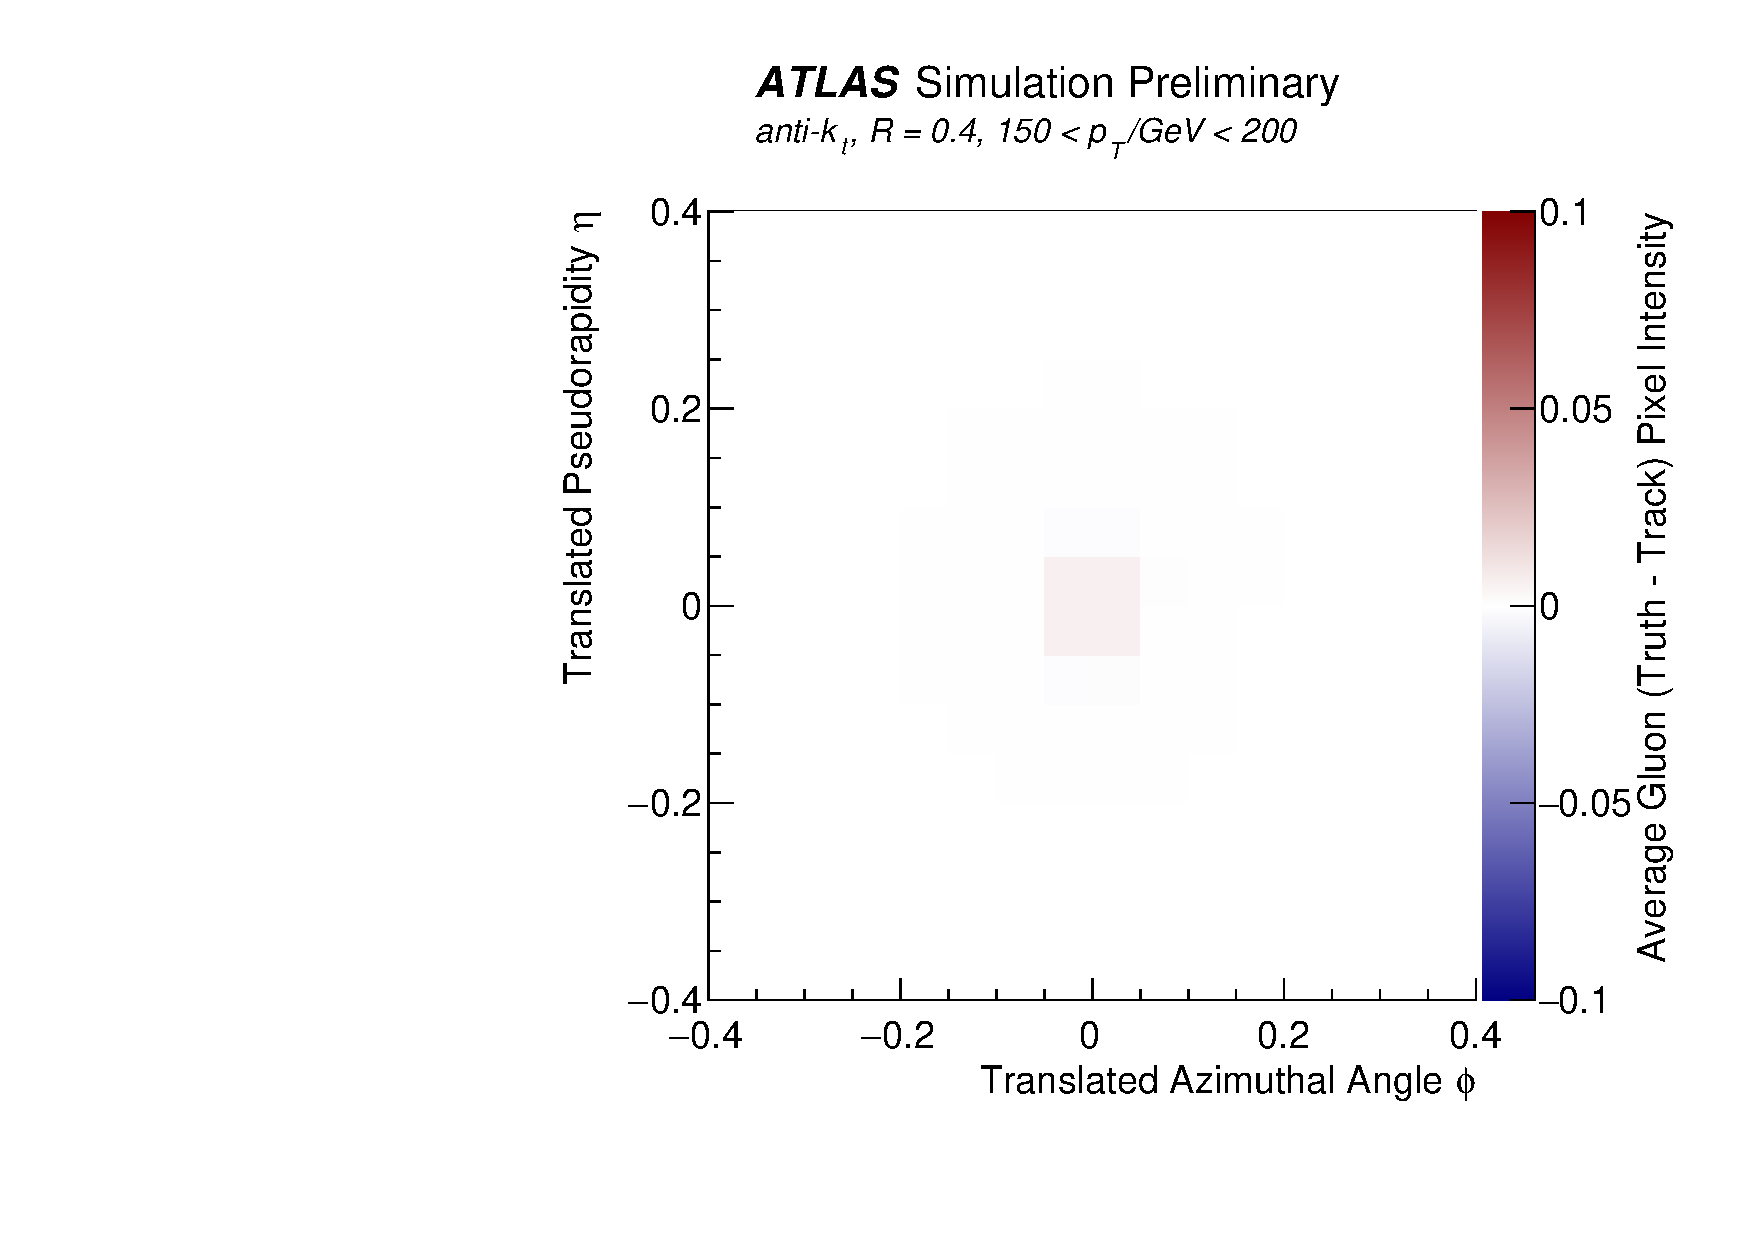
\includegraphics[width=0.31\textwidth]{figures/CNN/diff_gluon_truth_track.pdf}
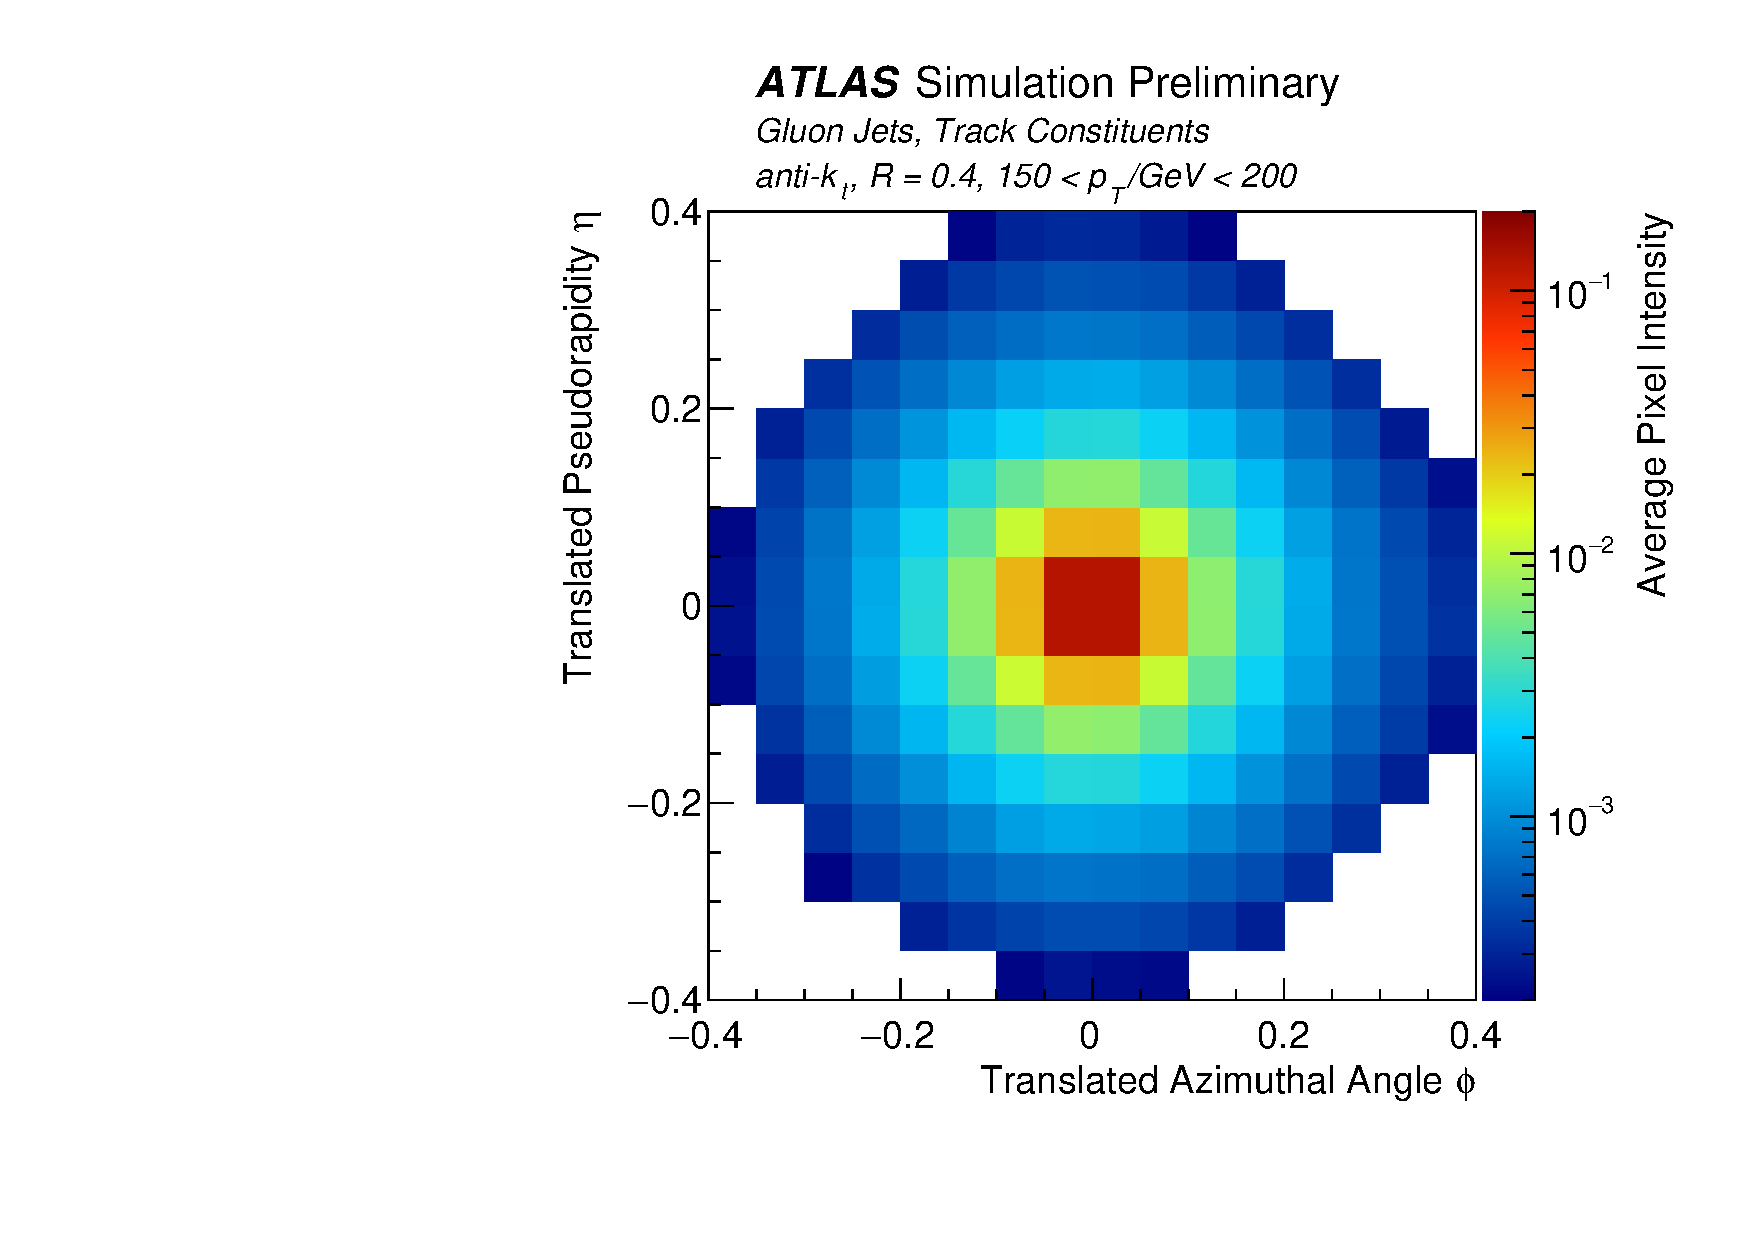
\includegraphics[width=0.31\textwidth]{figures/CNN/gluon_track.pdf}
\caption{The four corners show the average quark (upper) and gluon (lower) jet images, from true constituents, both charged and neutral, (left) and reconstructed tracks (right); the four plots on the edges show the difference between the adjacent plots, for example the top plot shows the difference between the average quark jet for stable particles and reconstructed tracks. Quark-jets are more collimated than gluon ones, and track images show slightly less central activity than in the true jet.}
\label{fig:cnn-avg:truthtrack}
\end{center}
\end{figure}

\begin{figure}[h!]
\begin{center}
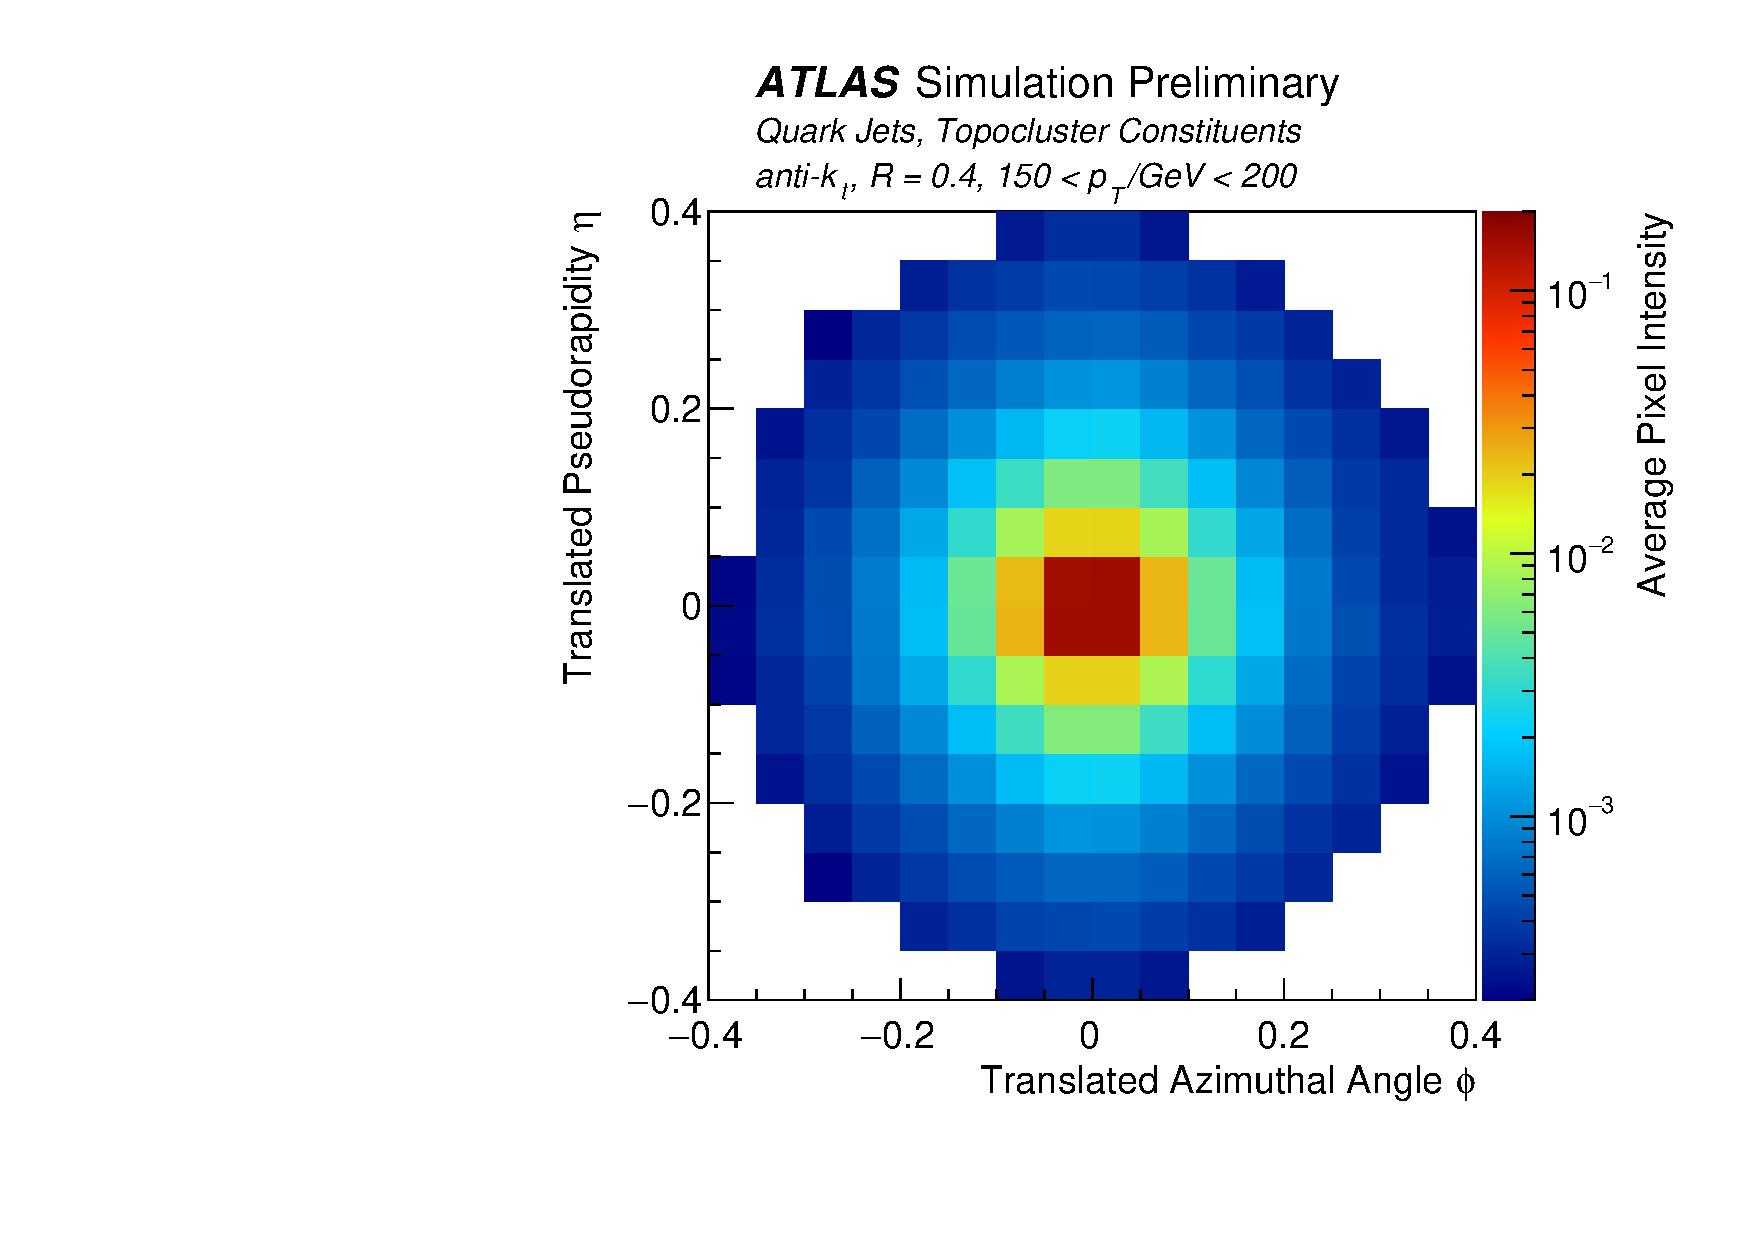
\includegraphics[width=0.31\textwidth]{figures/CNN/quark_cluster.pdf}
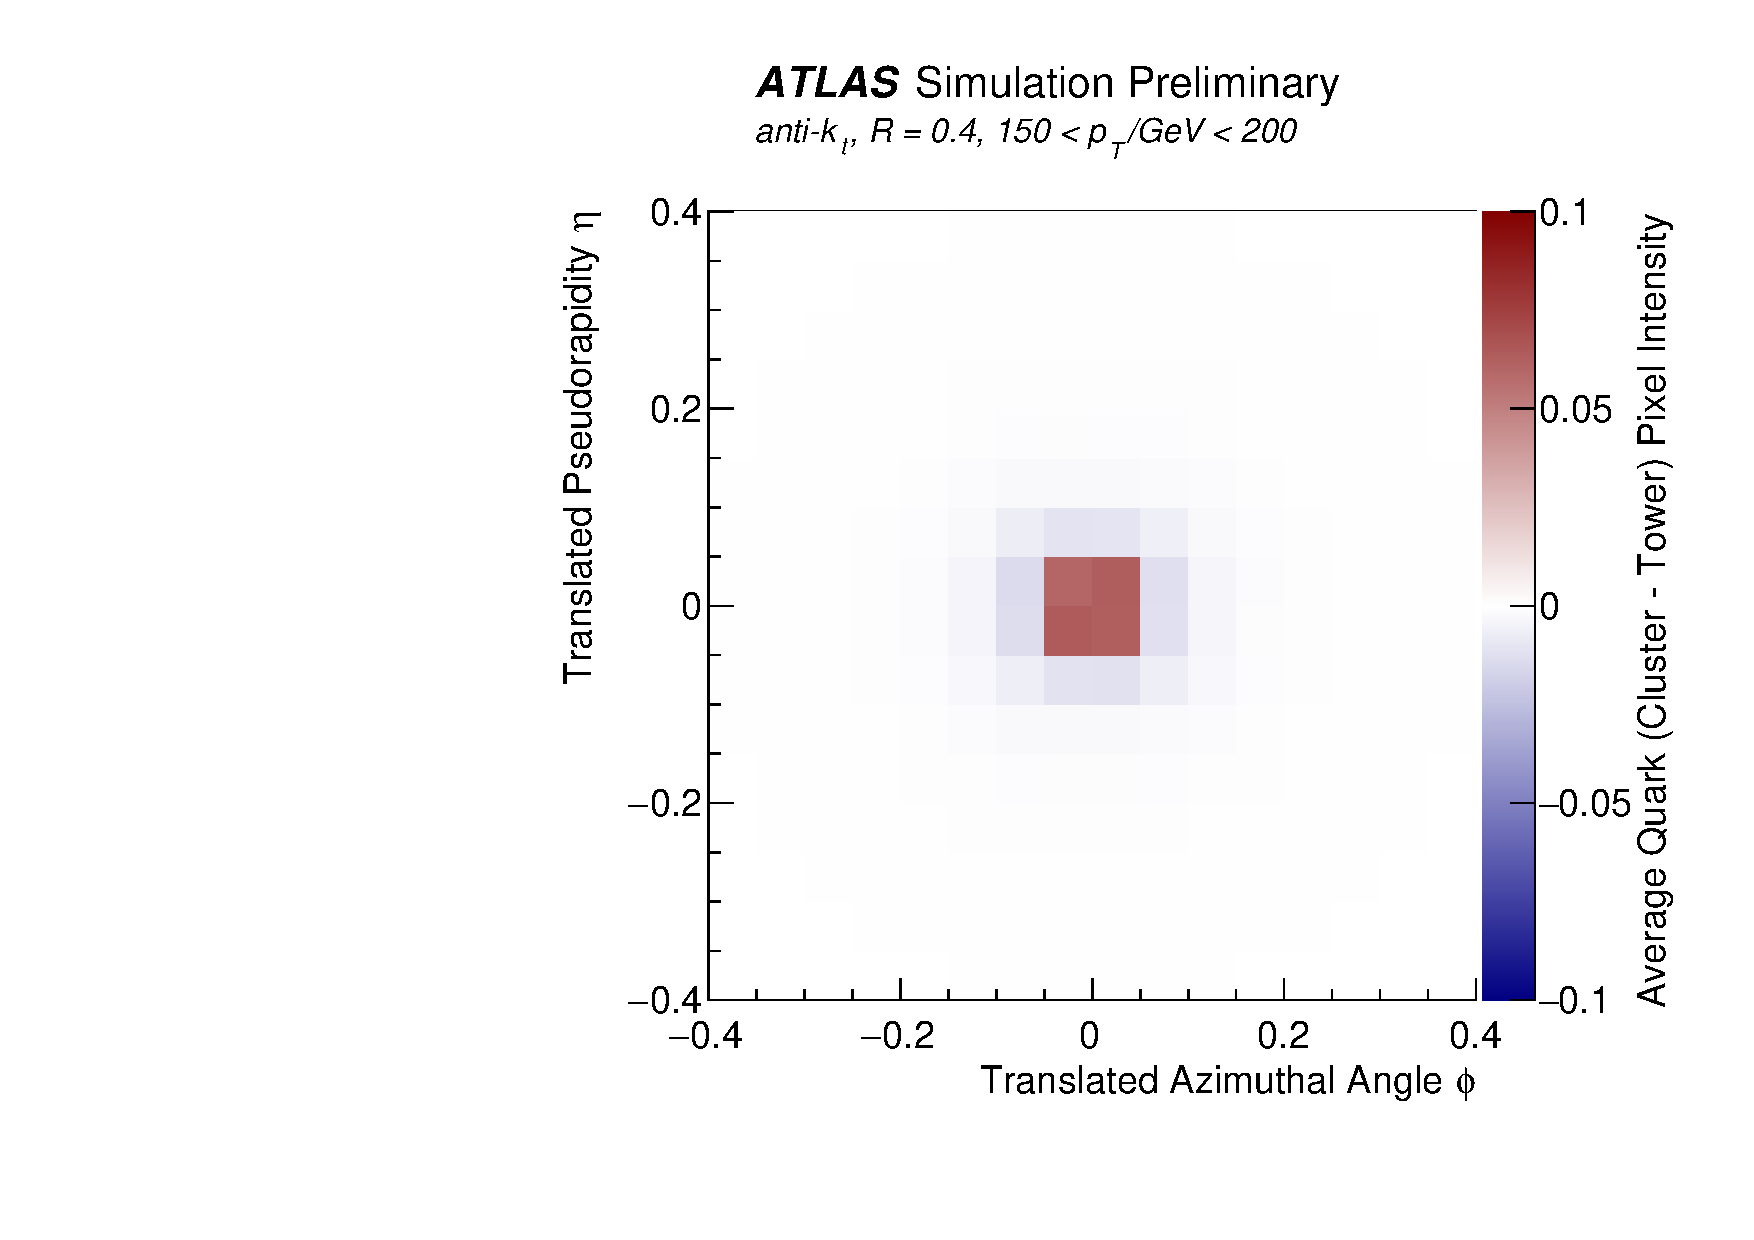
\includegraphics[width=0.31\textwidth]{figures/CNN/diff_quark_cluster_tower.pdf}
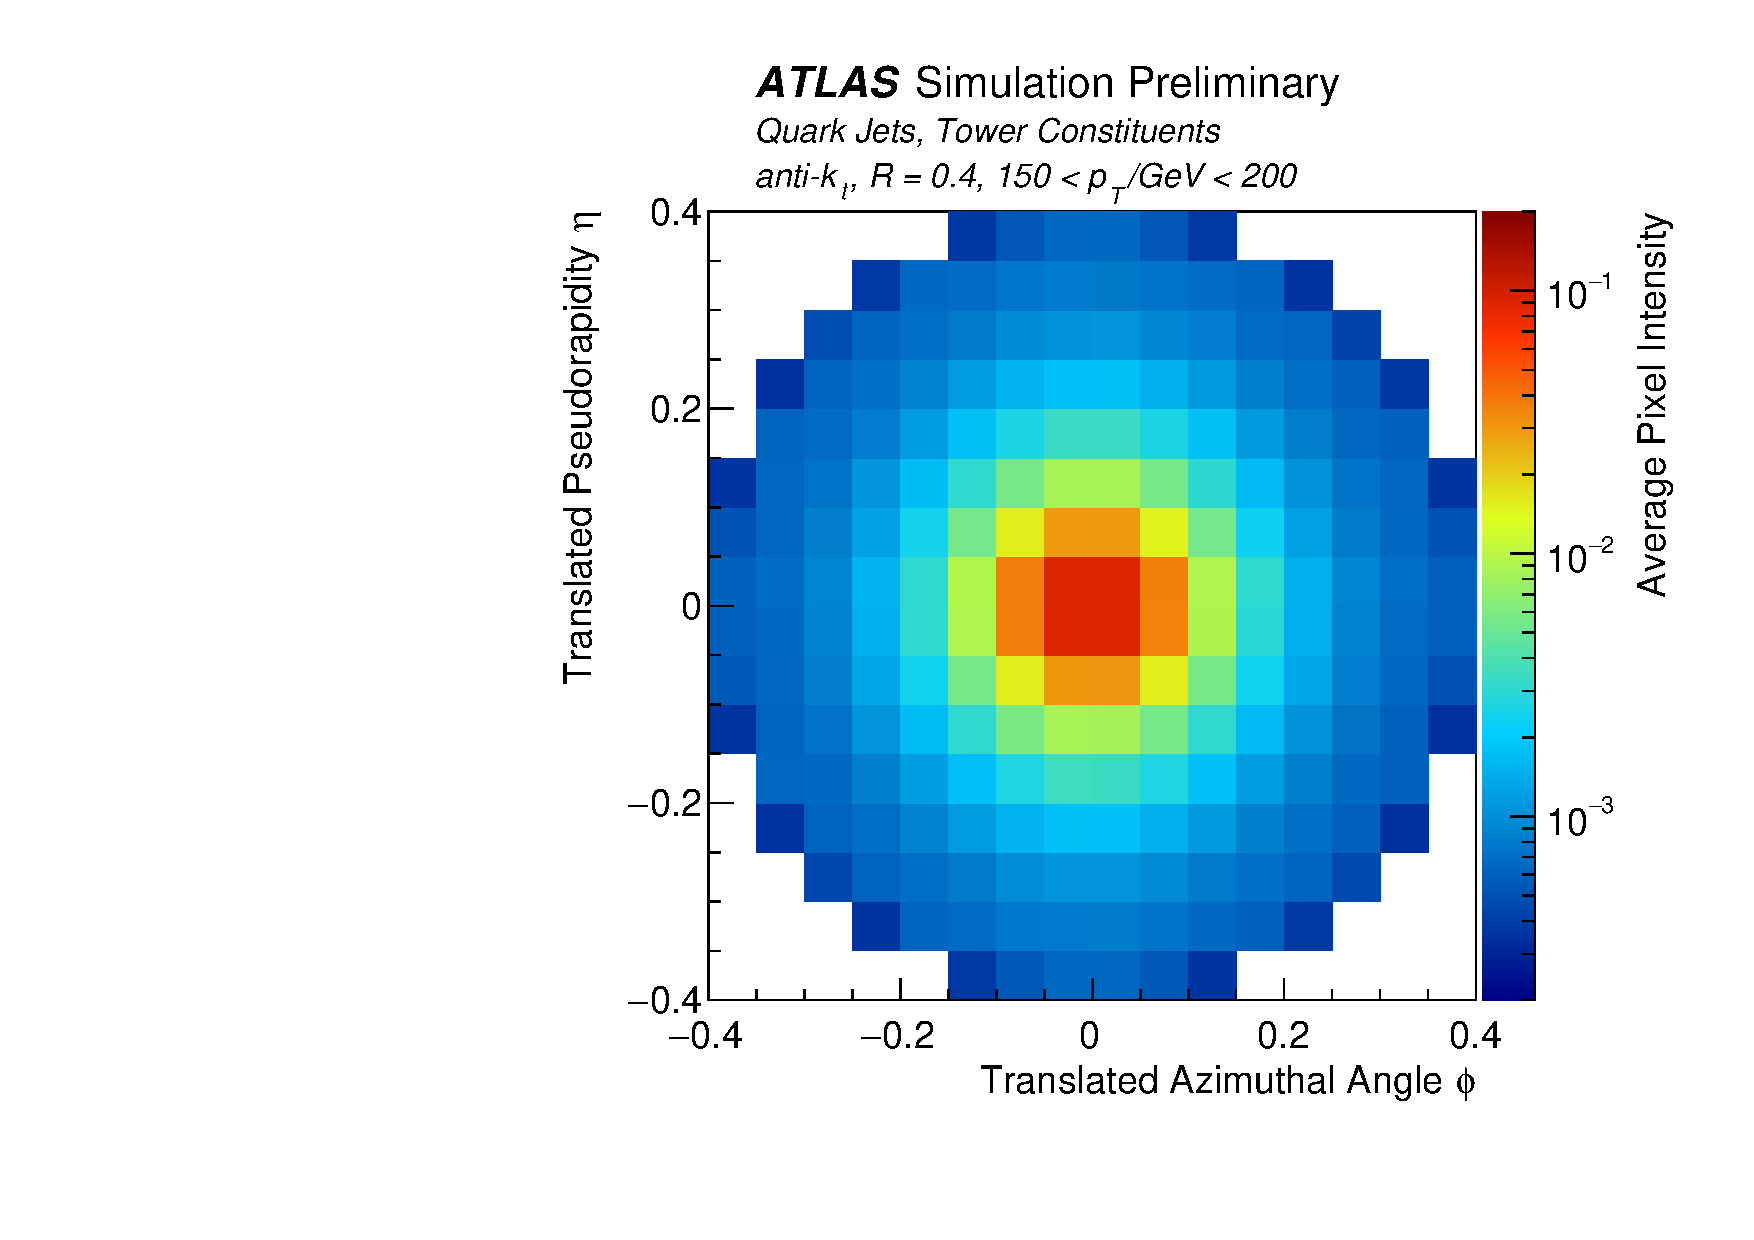
\includegraphics[width=0.31\textwidth]{figures/CNN/quark_tower.pdf}\\
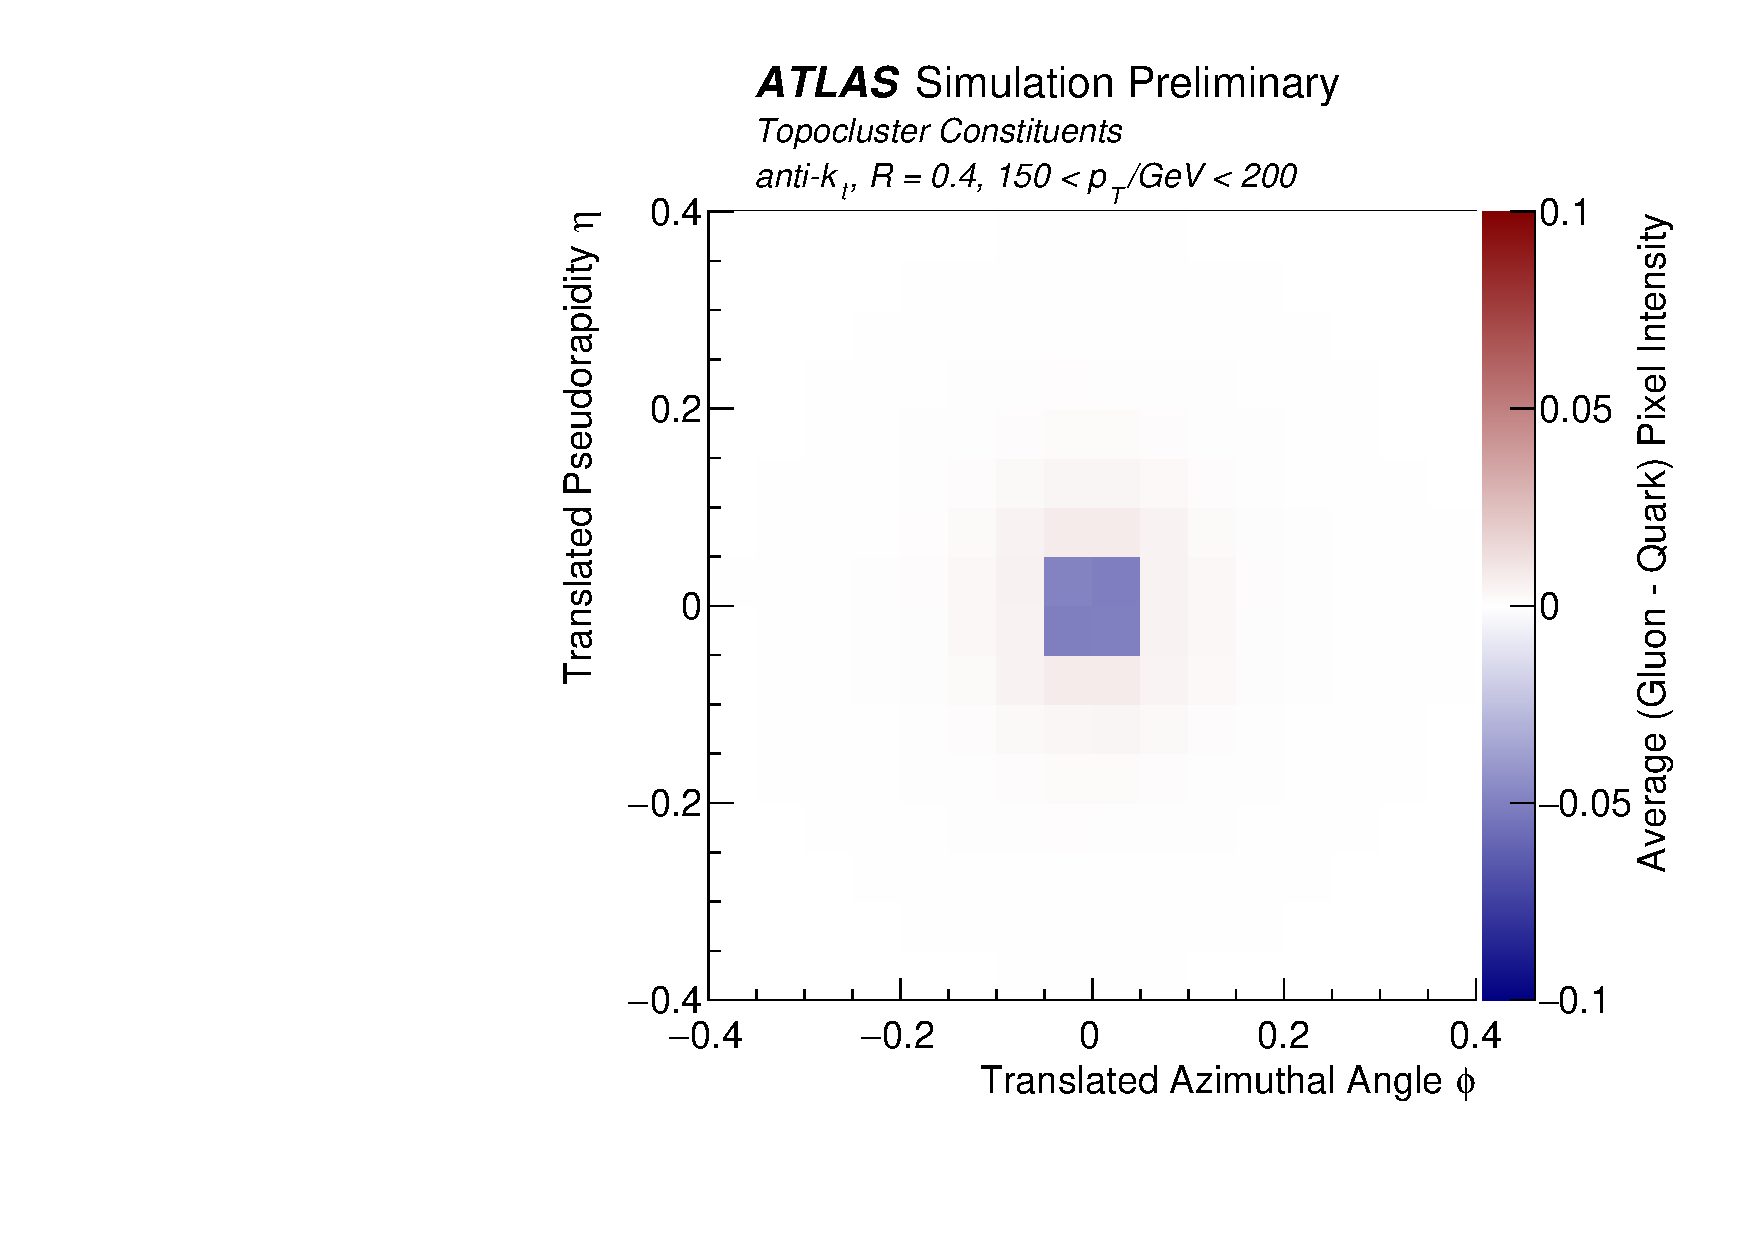
\includegraphics[width=0.31\textwidth]{figures/CNN/diff_cluster.pdf}\hspace{54mm}
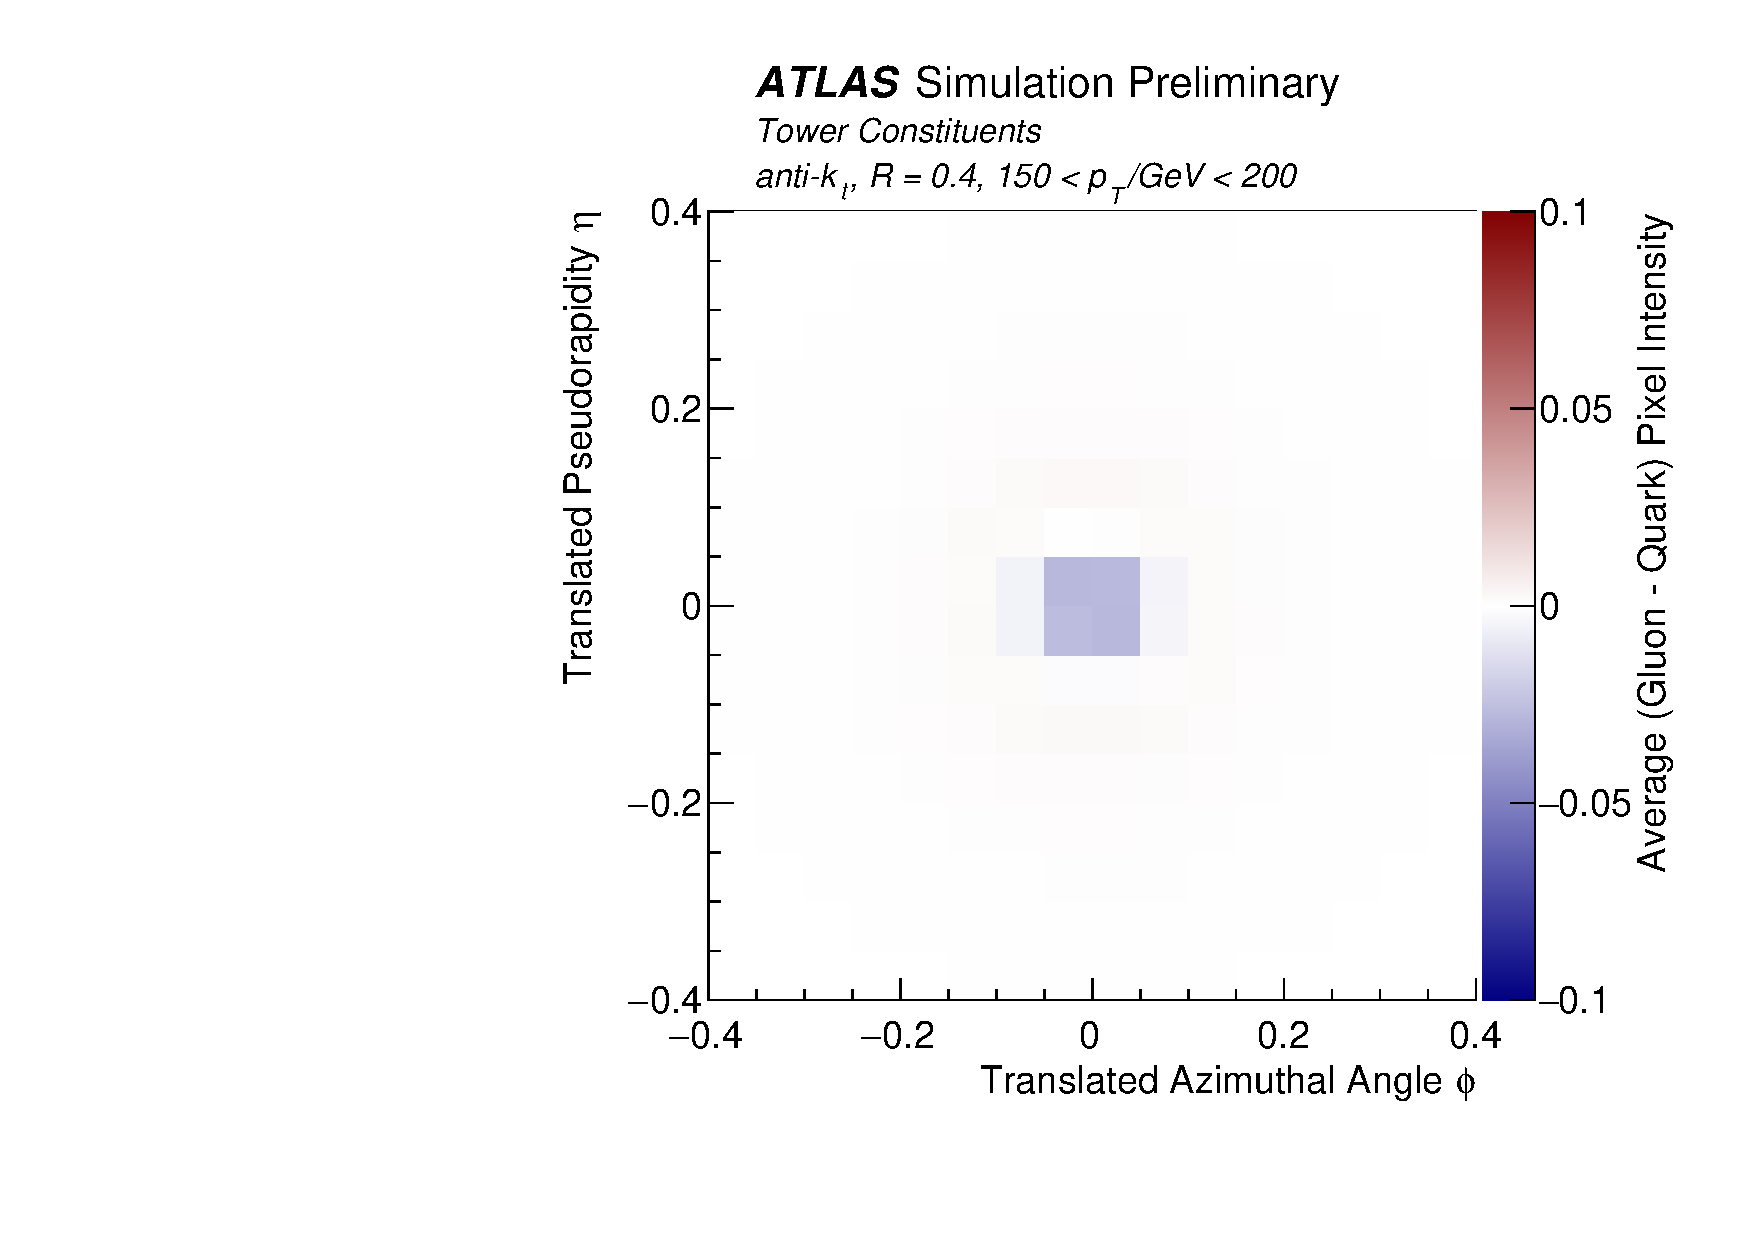
\includegraphics[width=0.31\textwidth]{figures/CNN/diff_tower.pdf}\\
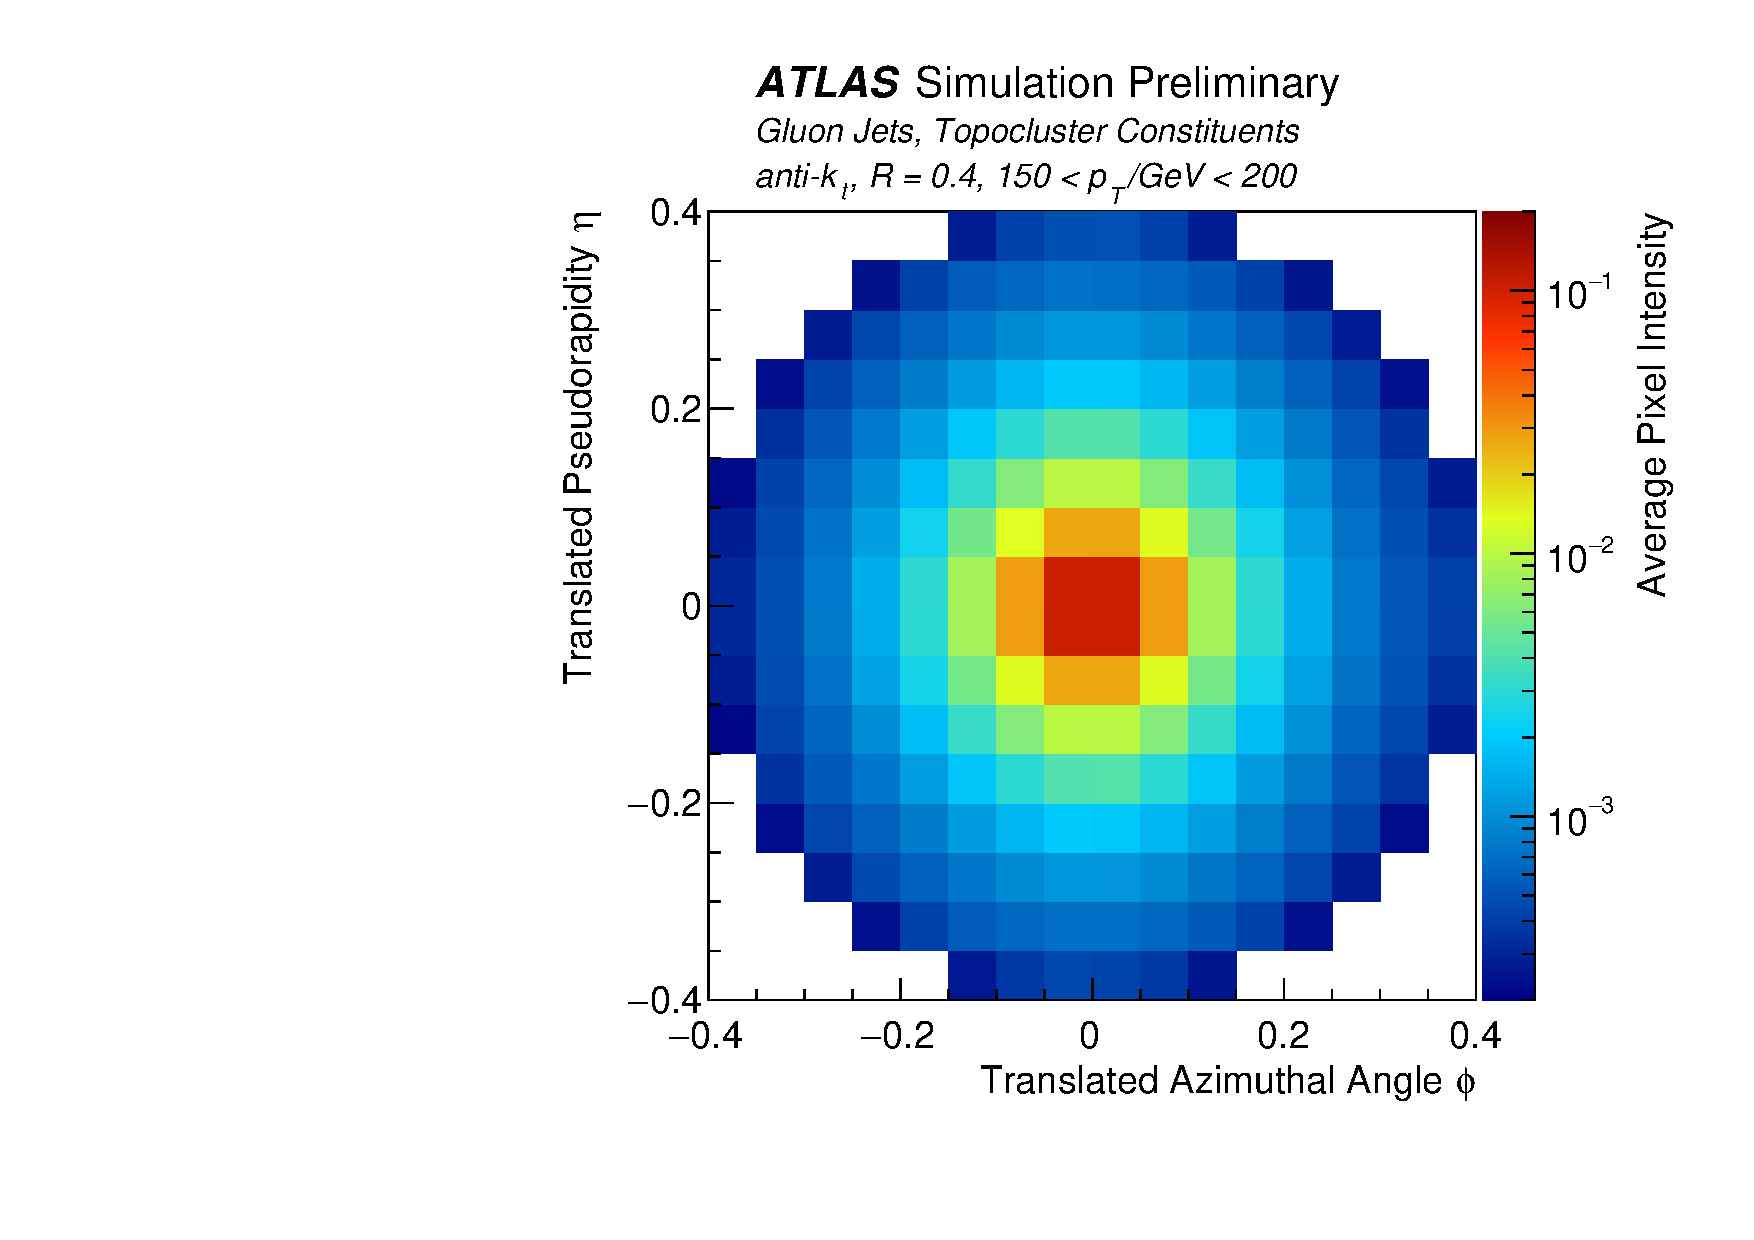
\includegraphics[width=0.31\textwidth]{figures/CNN/gluon_cluster.pdf}
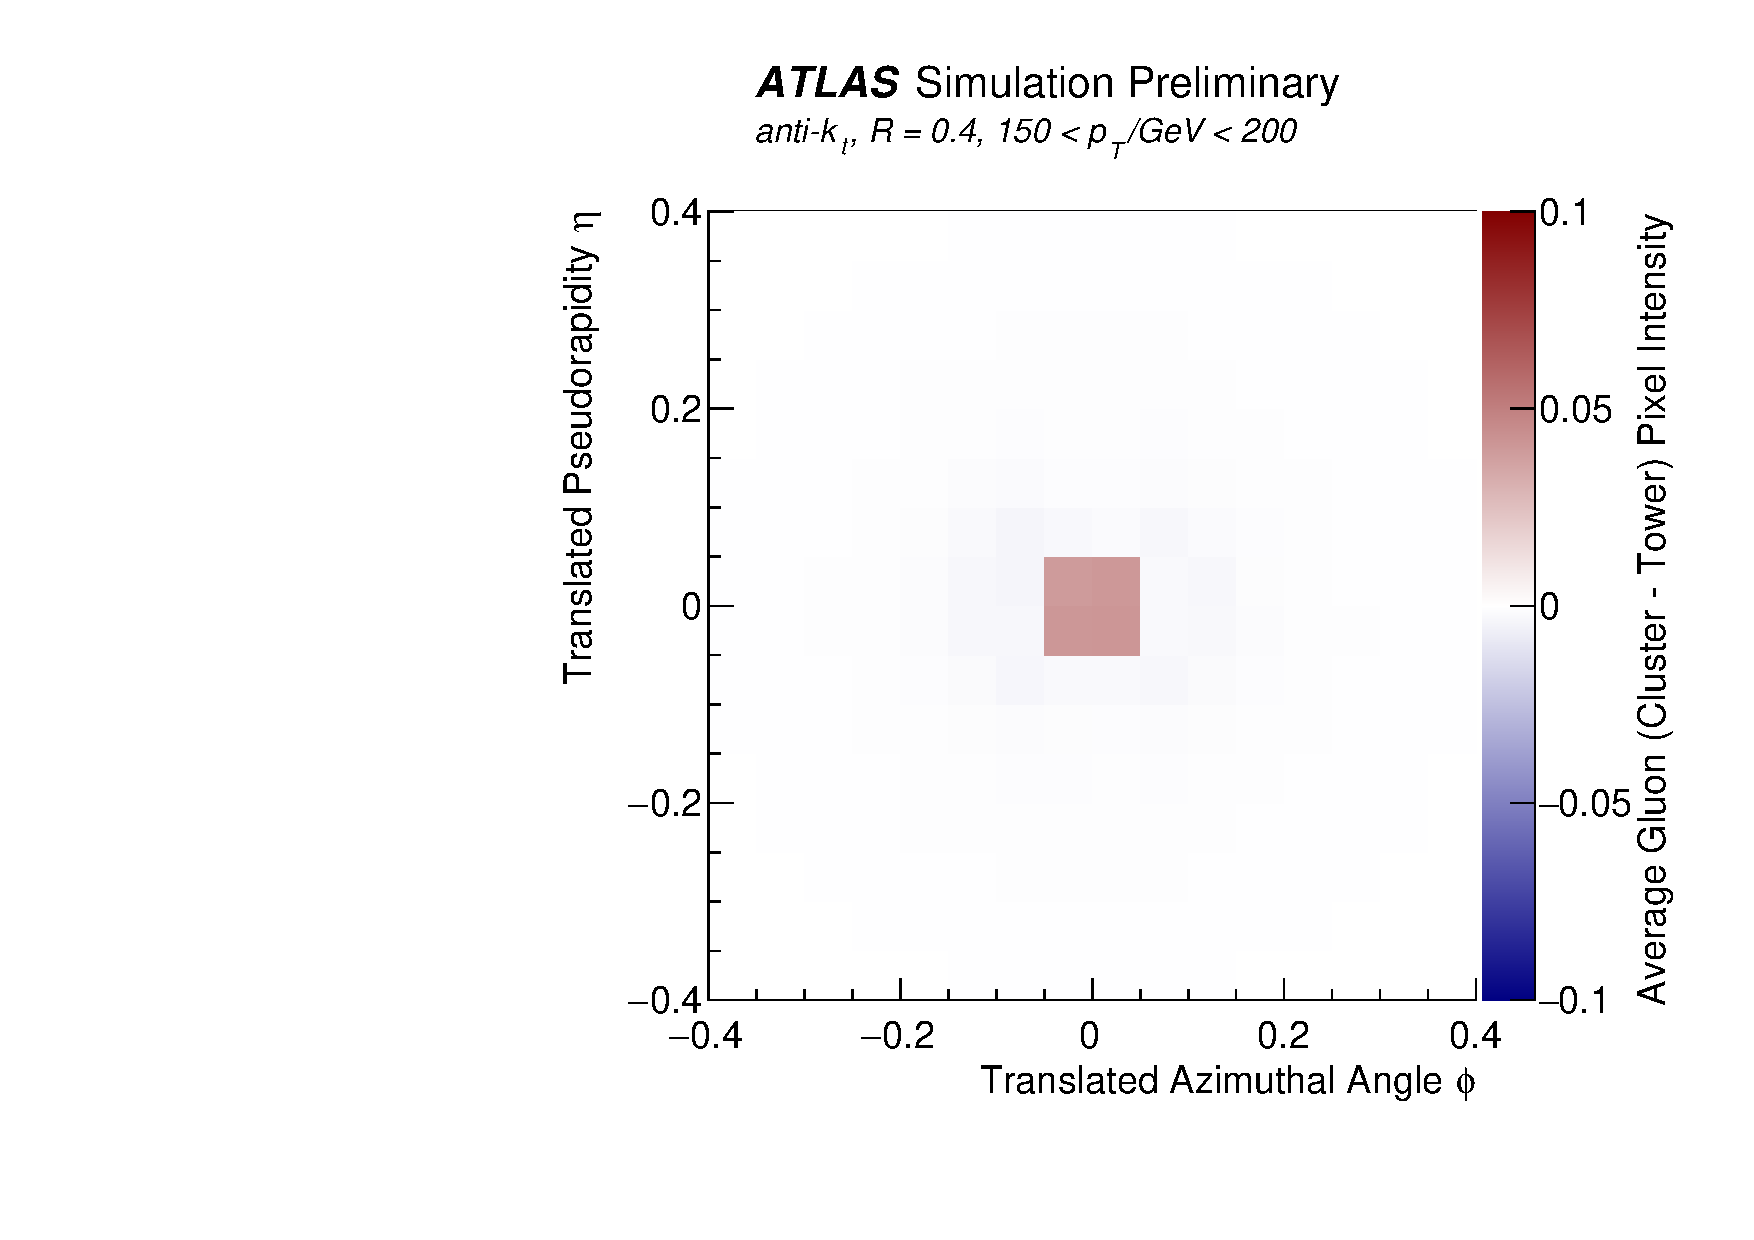
\includegraphics[width=0.31\textwidth]{figures/CNN/diff_gluon_cluster_tower.pdf}
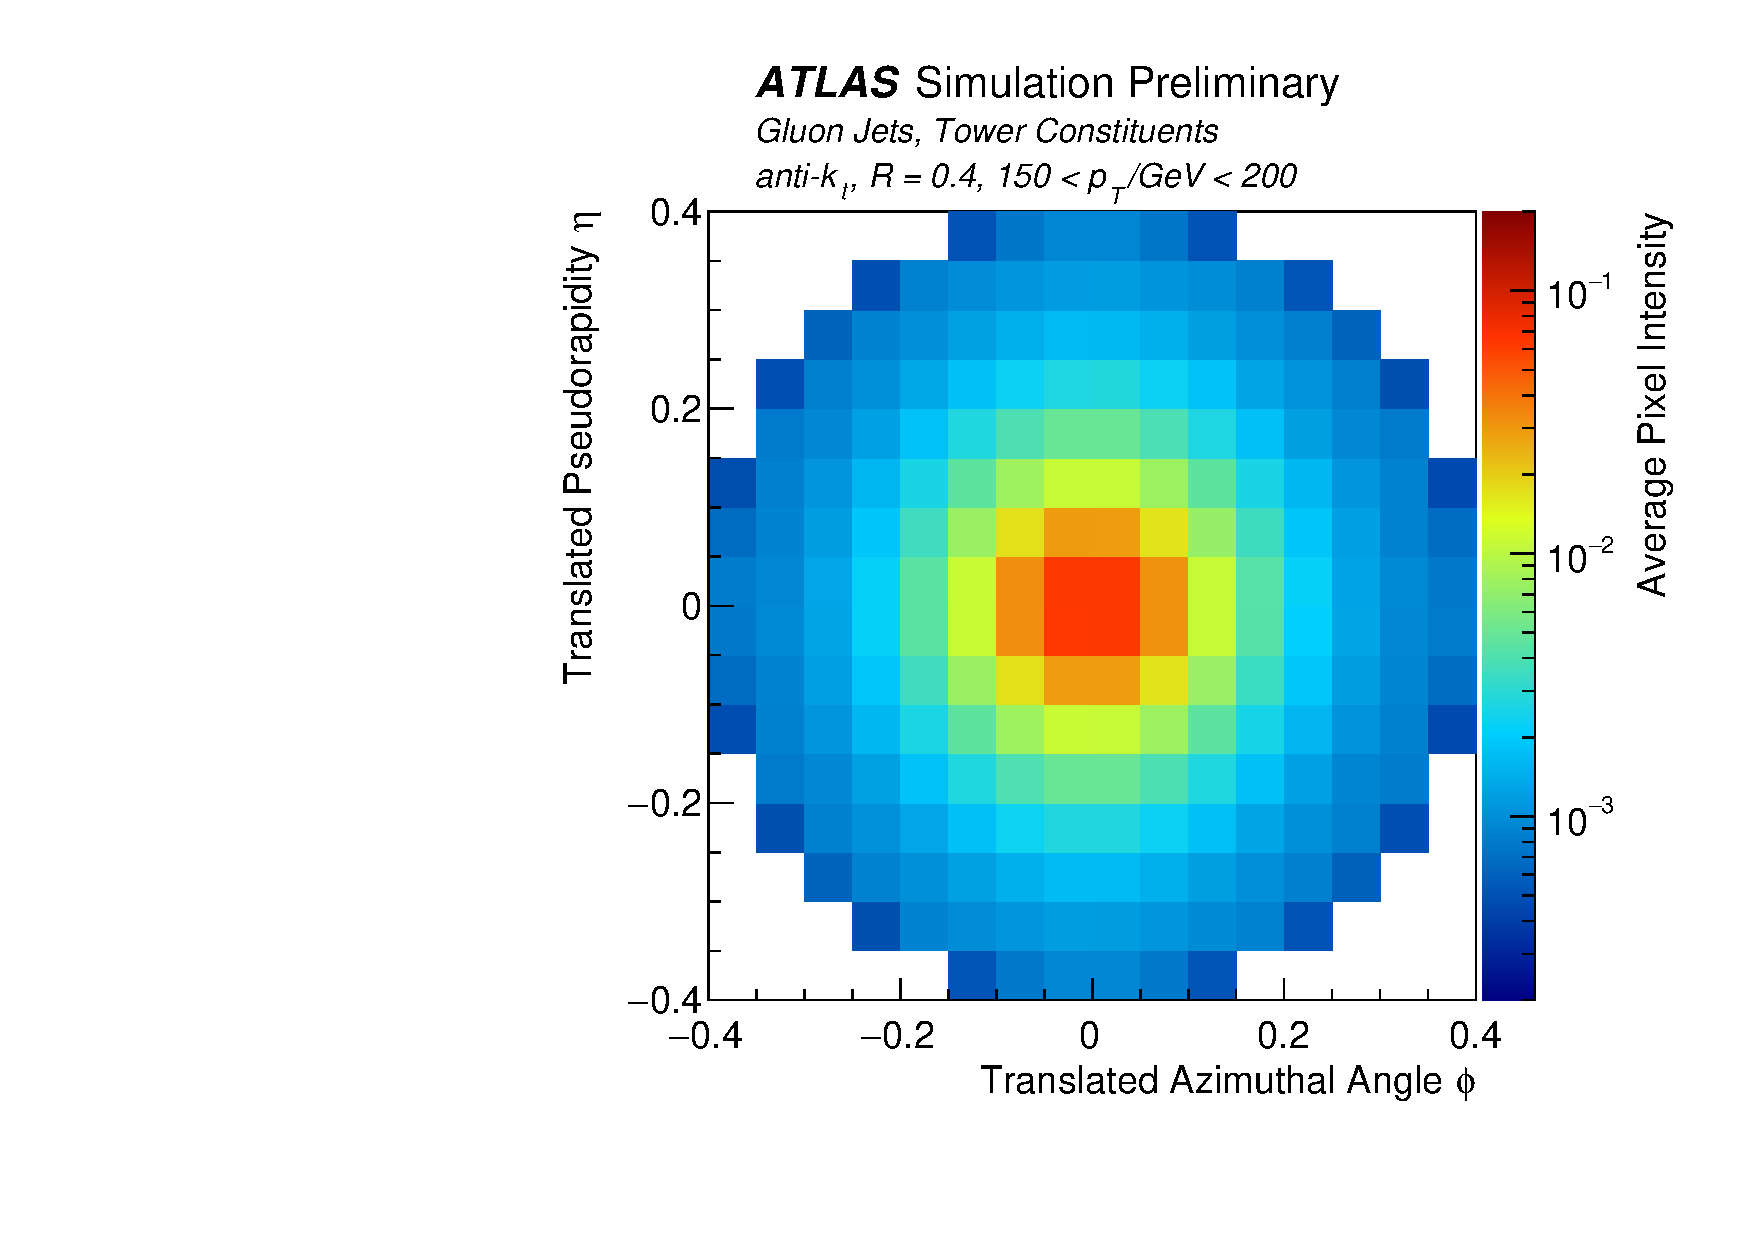
\includegraphics[width=0.31\textwidth]{figures/CNN/gluon_tower.pdf}
\caption{The four corners show the average quark (upper) and gluon (lower) jet images, from topo-clusters (left) and towers (right); the four plots on the edges show the difference between the adjacent plots, for example the top plot shows the difference between the average quark jet for topoclusters and towers. Quark-jets are more collimated than gluon ones, and topo-cluster images are more collimated than tower images.}
\label{fig:cnn-avg:clustertower}
\end{center}
\end{figure}

\clearpage

